\documentclass{jsarticle}

\usepackage{amsmath, amssymb, amsthm}
\usepackage{bm}
\usepackage[dvipdfmx]{graphicx}
\usepackage[dvipdfmx]{color}
\usepackage{wrapfig}
\usepackage{comment}
\usepackage{mathrsfs}
\usepackage{longtable}
\usepackage{here}
\usepackage{hhline}
\usepackage{ascmac}
\usepackage{braket}
\usepackage{hhline}
\usepackage{color}
% \usepackage{ccicons}
\usepackage[type={CC},modifier={by},version={4.0},]{doclicense}
\usepackage[all]{xy}
\usepackage[dvipdfmx,colorlinks=true,linkcolor=blue,filecolor=blue,urlcolor=blue]{hyperref}
\usepackage{atbegshi}
\ifnum 42146=\euc"A4A2
  \AtBeginShipoutFirst{\special{pdf:tounicode EUC-UCS2}}
\else
  \AtBeginShipoutFirst{\special{pdf:tounicode 90ms-RKSJ-UCS2}}
\fi


% \usepackage[color]{showkeys}
% \definecolor{refkey}{rgb}{0.15,0.8,0.2}
% \definecolor{labelkey}{rgb}{0.15,0.8,0.2}


%macro

\newcommand\id{}
\newcommand\cmt[1]{}

\newcommand\setN{\mathbb{N}}
\newcommand\setZ{\mathbb{Z}}
\newcommand\setQ{\mathbb{Q}}
\newcommand\setR{\mathbb{R}}
\newcommand\setC{\mathbb{C}}
\newcommand\setH{\mathbb{H}}

% \newcommand\subknot{\subset}
\newcommand\subknot[1]{{#1}^*}

\newcommand\Cl[1]{\overline{#1}}
\newcommand\Int[1]{\interior\Pare{#1}}

\newcommand\abs[1]{|#1|}
\newcommand\Abs[1]{\left|#1\right|}
\newcommand\pare[1]{(#1)}
\newcommand\Pare[1]{\left(#1\right)}
\newcommand\curl[1]{\{#1\}}
\newcommand\Curl[1]{\left\{#1\right\}}
\newcommand\squa[1]{[#1]}
\newcommand\Squa[1]{\left[#1\right]}
\newcommand\angl[1]{\langle#1\rangle}
\newcommand\Angl[1]{\left\langle#1\right\rangle}

\newcommand\transpose[1]{\,{\vphantom{#1}}^t\!#1}
\newcommand\E[1]{\!\,{\vphantom{#1}}^\exists #1}
\newcommand\A[1]{\!\,{\vphantom{#1}}^\forall #1}
\newcommand\Z[2]{\squa{#1,#2}_\mathbb{Z}}

\newcommand\colvec[1]{
    \begin{pmatrix}
        #1
    \end{pmatrix}
}
\newcommand\rowvec[1]{
    \begin{pmatrix}
        #1
    \end{pmatrix}
}

\newcommand\sfrac[2]{#1/#2}

\newcommand\od[2]{\frac{d #1}{d #2}}
\newcommand\dod[2]{\dfrac{d #1}{d #2}}
\newcommand\sod[2]{\sfrac{d #1}{d #2}}

\newcommand\pd[2]{\frac{\partial #1}{\partial #2}}
\newcommand\dpd[2]{\dfrac{\partial #1}{\partial #2}}
\newcommand\spd[2]{\sfrac{\partial #1}{\partial #2}}

\newcommand\LagD[1]{\frac{\mathrm{D} #1}{\mathrm{D} t}}
\newcommand\dLagD[1]{\dfrac{\mathrm{D} #1}{\mathrm{D} t}}
\newcommand\sLagD[1]{\sfrac{\mathrm{D} #1}{\mathrm{D} t}}

% \newcommand\nCr[2]{{}_{#1} \hspace{-0.1em} {C} _{#2} \hspace{0.1em}}
\newcommand\nCr[2]{\binom{#1}{#2}}
\newcommand\nPr[2]{{}_{#1} \hspace{-0.1em} {P} _{#2} \hspace{0.1em}}
\newcommand\const{=(const.)}
\newcommand\Def{\overset{\mathrm{def}}{\Longleftrightarrow}}
\newcommand\simarrow{\overset{\scalebox{1.29}[0.8]{$\sim$}}{\to}}
\newcommand\nsimarrow{\overset{\scalebox{1.29}[0.8]{$\nsim$}}{\to}}

\DeclareMathOperator*{\spn}{span}
\DeclareMathOperator{\tr}{tr}
\DeclareMathOperator{\rk}{rank}
\DeclareMathOperator{\nl}{null}
\DeclareMathOperator{\grad}{grad}
\let\div\relax
\DeclareMathOperator{\div}{div}
\DeclareMathOperator{\rot}{rot}
\DeclareMathOperator{\supp}{supp}
\DeclareMathOperator*{\conv}{Conv}
\DeclareMathOperator*{\Res}{Res}
\DeclareMathOperator{\interior}{Int}
\DeclareMathOperator{\closure}{Cl}

\DeclareMathOperator{\N}{\mathfrak{n}}


\newcommand\Quote[1]{``#1''}

\newcommand\I{I}
\newcommand\II{I\hspace{-0.1em}I}
\newcommand\III{I\hspace{-0.1em}I\hspace{-0.1em}I}

%theorem
\theoremstyle{definition}% default
\newtheorem{thm}{定理}
\newtheorem*{thm*}{定理}
\newtheorem{defn}[thm]{定義}
\newtheorem*{defn*}{定義}
\newtheorem{lem}[thm]{補題}
\newtheorem*{lem*}{補題}
\newtheorem{prop}[thm]{命題}
\newtheorem*{prop*}{命題}
\newtheorem{exmp}{例}
\newtheorem*{exmp*}{例}
\newtheorem*{rem}{注意}
\newtheorem*{note}{ノート}
\renewcommand\proofname{\textbf{証明}}

\newcommand\UC{\textcolor{red}{(執筆中です)}}

\makeatletter
\c@MaxMatrixCols=12
\makeatother

\allowdisplaybreaks[4]


\title{NURBS多様体による形状表現}
% \author{堀川由人}
\author{\href{https://hyrodium.github.io/Profile}{堀川 由人}}

\begin{document}
\maketitle
\vspace{2em}
\begin{figure}[H]
	\centering
    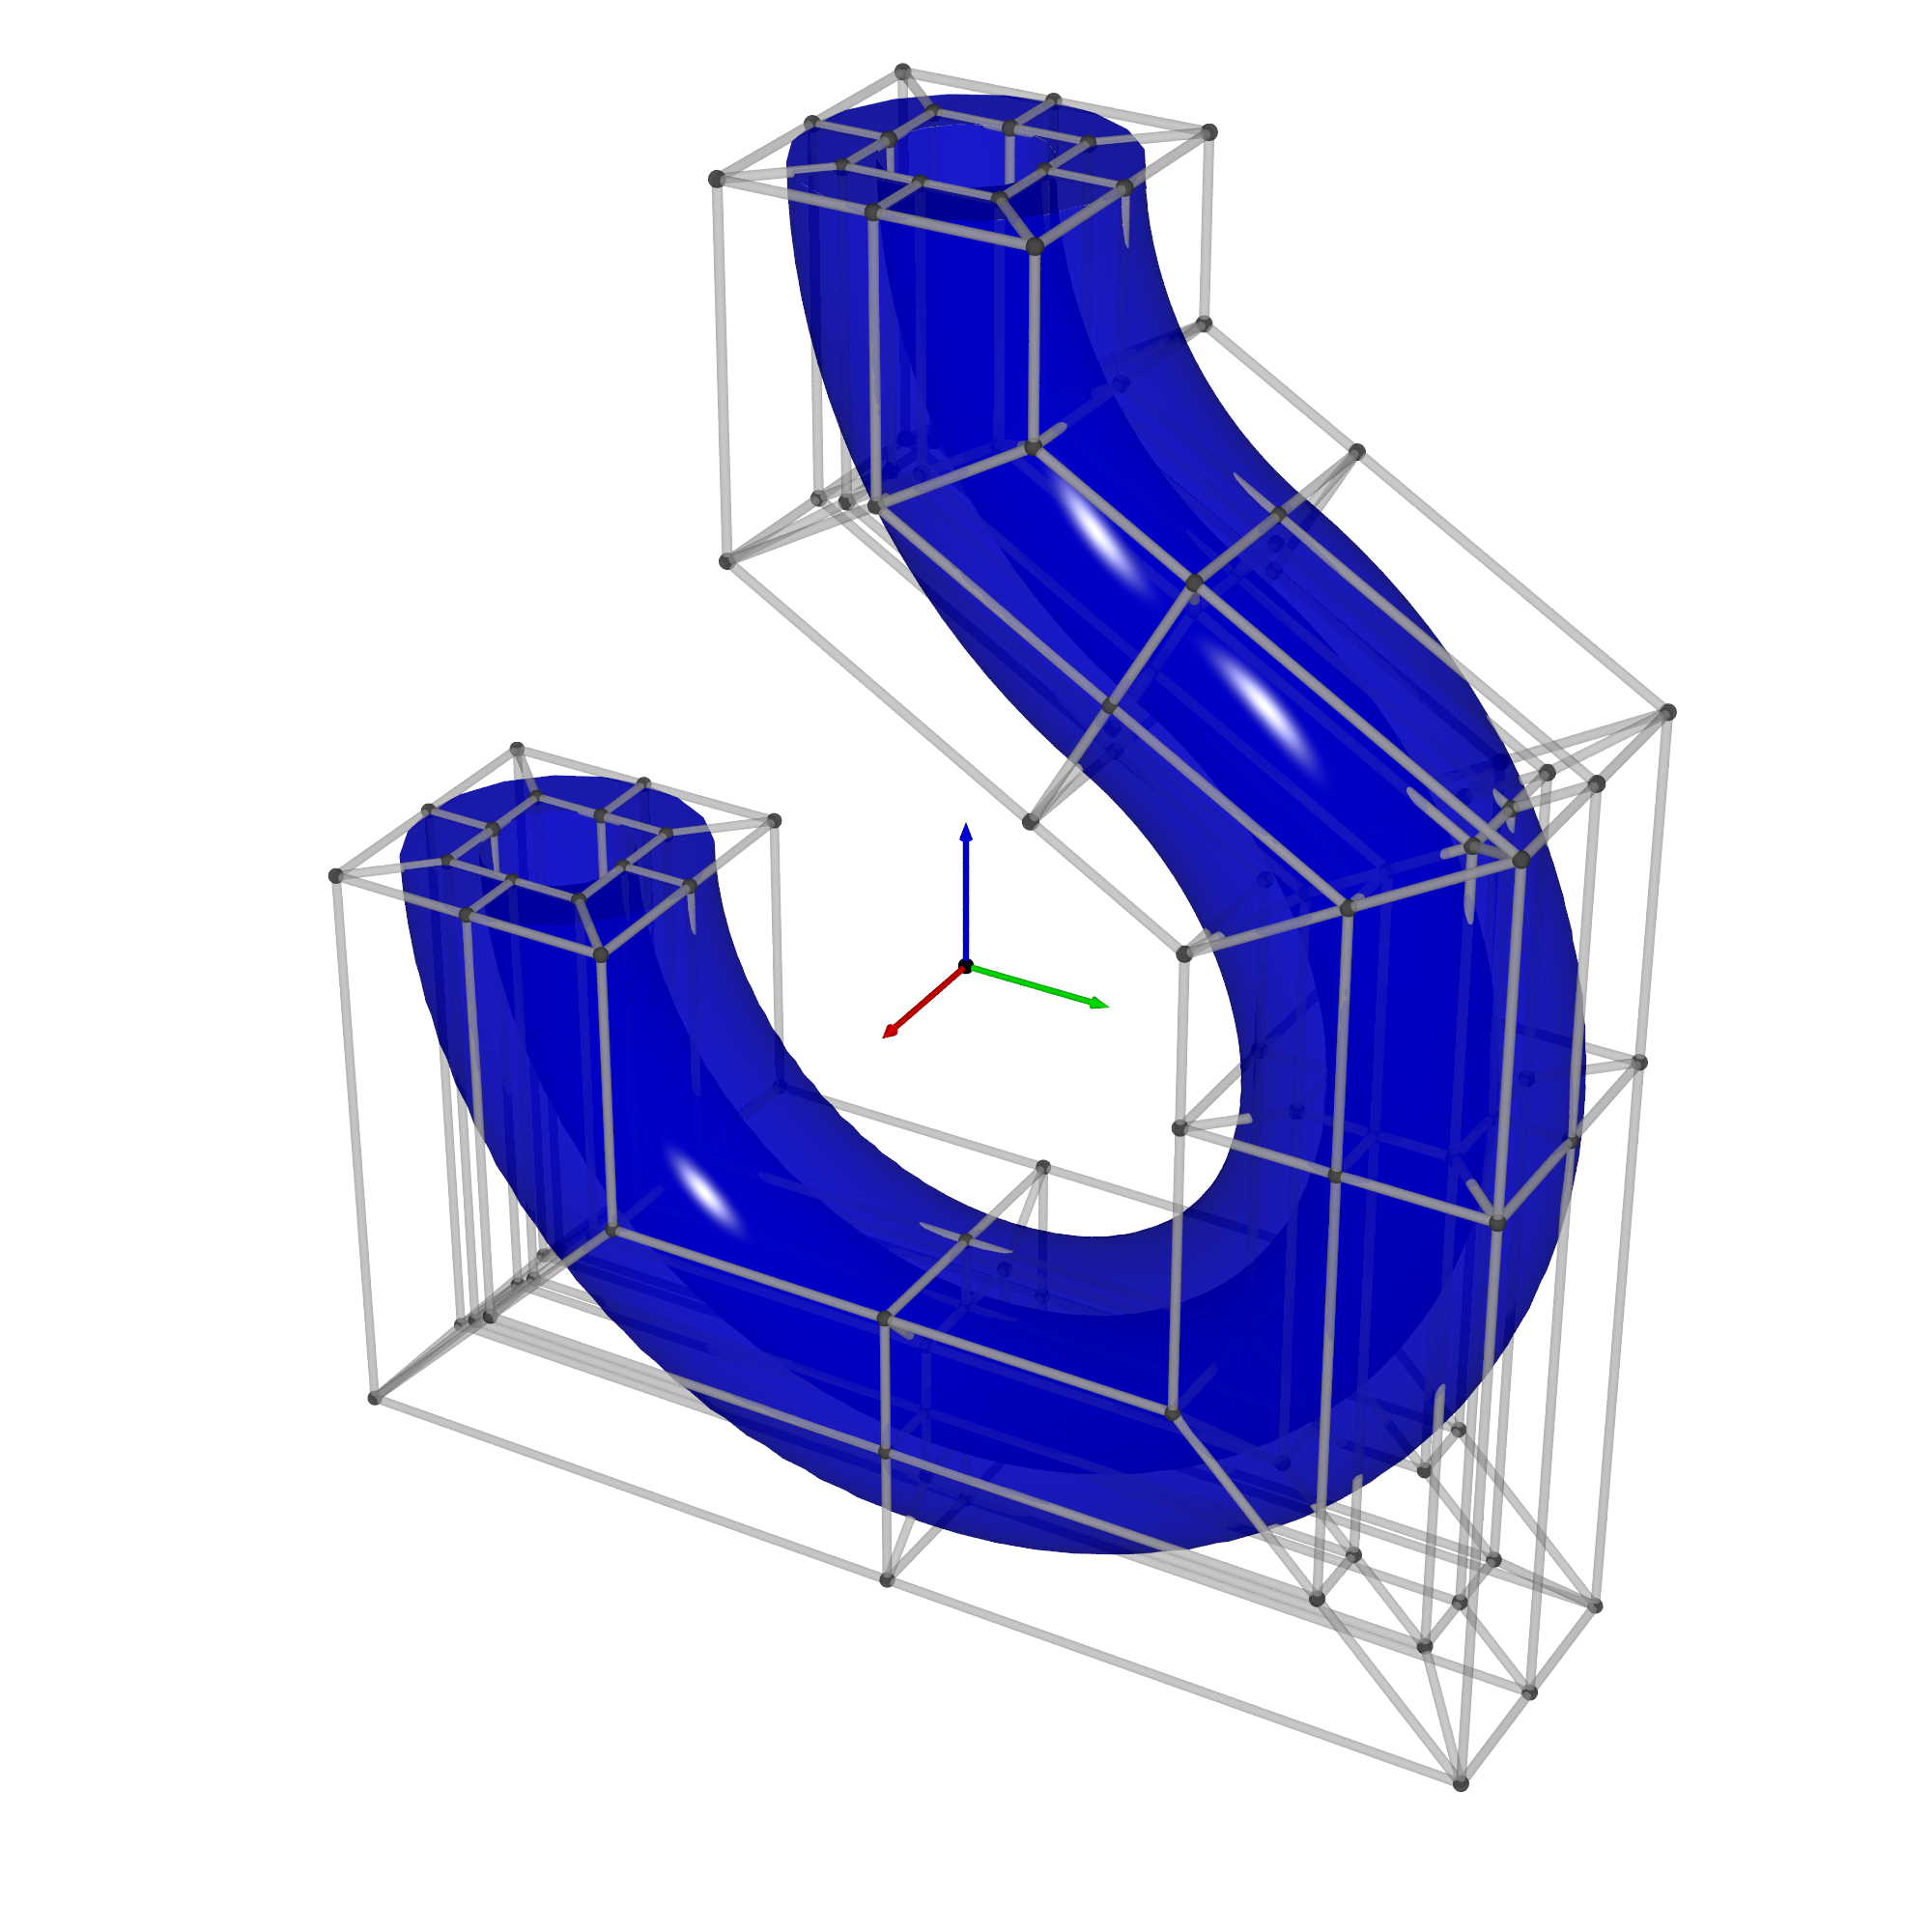
\includegraphics[width=160mm]{cover.png}
\end{figure}

\thispagestyle{empty}
\newpage

% \section{概要}
\section*{はじめに}
\pagenumbering{roman}
NURBS(Non-uniform Rational B-spline)はコンピュータ上で物体の形状を表現するために開発された手法である.
NURBSを用いれば
% \begin{itemize}
%     \item 次元 $d$
%     \item ノット列 $\bm{k}_1,\dots,\bm{k}_d$
%     \item 次数 $p_1,\dots,p_d$
%     \item 重み $w_{i_1\cdots i_d}$
%     \item 制御点 $\bm{a_{i_1\cdots i_d}}$
% \end{itemize}
\begin{tabbing}
    \hspace{5.2mm} \= \hspace{20mm} \= \hspace{30mm} \kill
    \> \labelitemi \, 次元 \> $d$ \\
    \> \labelitemi \, ノット列 \> $\bm{k}^1,\dots,\bm{k}^d$ \\
    \> \labelitemi \, 次数 \> $p^1,\dots,p^d$ \\
    \> \labelitemi \, 重み \> $w_{1\cdots 1},\dots,w_{n^1\cdots n^d}$ \\
    \> \labelitemi \, 制御点 \> $\bm{a}_{1\cdots 1},\dots,\bm{a}_{n^1\cdots n^d}$
\end{tabbing}
を定めるだけで物体の形状を決める事が可能で, かつその表現は非常に柔軟である.
形状表現の類似手法として, B\'ezier曲線/曲面, B-spline曲線/曲面などがあるが, これらは全てNURBSで表現可能な形状である.
この意味で, NURBSは一般性, 汎用性の高い手法であり, こうした利点がのコンピューター上の形状表現で利用されている理由である.


% 前章で述べたように, 本研究ではNURBSを用いて表現された古典弾性体およびひずみ勾配弾性体を解析対象として, それらに対するIsogeometric Analysis(IGA)の実装を目的としている.
% IGAでは弾性体の形状をNURBSによって幾何的に性格んな形状として表現することによって

% 従来の有限要素法では, 多くの場合において弾性体は単体分割による近似が行われ, その近似が幾何的に厳密に表現できない事に起因する誤差が発生する.
% それに対しIGAでは, 弾性体をNURBSで表現することによって, 近似ではなく厳密に物体形状を表現することができる.
% さらに, IGAではNUBRSを弾性体の形状表現だけでなく, Galerkin法に基づく弱形式解析に用いるための基底関数としての役割も担うことになる.

% 以上を踏まえ, 本章では弾性体の形状を正確に表現する手法のNURBSについて, B\'ezier曲線などとの関係にも触れながら, 定義とその性質の解説を行う.

% Isogeometric Analysisにおいて, NURBSは弾性体を表現するための手法であると同時に, Galerkin法による弱形式解析に用いる基底関数としての役割も持つ.

NURBSの制御点を適切に削減できるよう一般化したものとしてT-splineもあるが, 本文章では簡単な紹介に留める.
なお, NURBS「多様体」と書いたのは単に曲線や曲面の一般化程度の意味合いであって, 多様体論の知識とかは必要としない.

\section*{参考文献}
NURBSは「物体の形状表現」という工学への応用が重視される道具であるから, 数学的に厳密な議論に立ち入らない書籍が多く, 記述が具体的過ぎて読みにくいものも多い.
そのため, NURBSについて数学的にちゃんと書かれている和書は私の知る限り存在しない.
以下に幾つかのNURBSに関連した書籍を挙げる.
\begin{itemize}
    \item Geometric Modeling with Splines: An Introduction, [Elaine Cohen \textit{et al.}] (2001) \\
    数学的に厳密かつ一般的に書かれている.
    本文章中の定理の殆どはこれにも載っている.
    B-splineによる内挿や, 発展的な形状表現についての記述もある.
    図も美しく, 大変おすすめ.
    \item The NURBS Book 2nd Edition [Les Piegl, \textit{et al.}] (1997) \\
    NURBSの使い方に主眼を置いて書かれている本. 入門書としてよく参照される.
    \item An Introduction to NURBS: With Historical Perspective [David F. Rogers] (2001) \\
    歴史的背景や擬似コードも記載されている.
    % \item Spline Functions: Basic Theory \\
    % 形状表現ではなく, スプライン関数による補間などを扱った書籍.
    % 初学者向けではない.
    \item 3Dグラフィックスのための数学入門 クォータニオン・スプライン曲線の基礎 [郡山彬ほか] (2015) \\
    NURBSについて書かれた最近の和書は少なく, その意味で貴重である.
    しかし高校数学の復習から四元数による回転も扱っているため, どうしてもNURBSに関連した記述は限られてしまっている.
    \item 情報科学 CAD/CAMにおける曲線曲面のモデリング [穂坂衛ほか] (1996) \\
    B-spline曲線をCox-de Boorの漸化式で定義せずに, B\'{e}zier曲線を区分的に繋げたものとして導入している.
    本文章で扱わなかった, 曲面の干渉の話題もある.
    \item NURBS ― 射影幾何学から実務まで [GERALD E.FARIN, 原孝成ほか] (2001) \\
    射影幾何や円錐曲線などの話題もあり, 導入が独特であるように思う.
    % \item CAD・CG技術者のためのNURBS早わかり \\
    % 読み物調で, 語り口に少し癖がある.
    % 感性の合う人には感覚を掴むのに良いのかも知れない.
    % \item CAD・CG技術者のための実践NURBS \\
    % ページ数の割に基本的な話に終始している.
\end{itemize}

% \newpage

\section*{記号}
以下に幾つかの記号の注意をまとめる.
\begin{tabbing}
    \hspace{5.2mm} \= \hspace{35mm} \= \hspace{1000mm} \kill
    \> \labelitemi \, $f:A\to B;a\mapsto b$ \> 写像$f$の始域と終域, 元の対応を表す. \\
    \> \labelitemi \, $\setN$ \> 自然数全体の集合. $\setN$は$0$を含むとする. \\
    \> \labelitemi \, $\Z{i}{j}$ \> $i$から$j$までの整数の集合. $\Z{i}{j}=\Set{i,i+1,\dots,j-1,j}=\Squa{i,j}\cap\setZ$. \\
    \> \labelitemi \, $\#S$ \> 集合$S$の元の個数. 本文章では有限集合に対してのみこの記号を使う. \\
    \> \labelitemi \, $C^{r}(U)$ \> $U$上の関数のうち, $r$階導関数が連続なもの全体の集合. $C^0$は単に連続関数. \\
    \> \labelitemi \, $A\subset B$ \> 集合$A,B$の包含関係. 真部分集合とは限らない. \\
    \> \labelitemi \, $\Cl{A}$ \> 集合$A$の閉包. \\
    \> \labelitemi \, $\conv(A)$ \> 集合$A$の凸包. \\
    \> \labelitemi \, $\supp(f)$ \> 関数$f:U\to\setR$の台. $\supp(f)=\Cl{\Set{x\in U|f(x)\neq 0}}$で定義される.
\end{tabbing}



\section*{この文章について}
図は\href{https://www.coreldraw.com}{CorelDRAW}, \href{https://juliagraphics.github.io/Luxor.jl/stable/}{Luxor (Julia package)}, \href{https://www.wolfram.com/mathematica/}{Mathematica}, \href{http://www.povray.org/}{POV-Ray}を使って作成した.
可能な限り図には\href{https://www.desmos.com/}{Desmos graphing calculator}へのリンクを付けており, インタラクティブに動かして理解が進むようにした.
このpdfファイルは\LaTeX で作成した.
この文章のライセンスは(CC BY 4.0)とする.
\doclicenseThis

\tableofcontents

\newpage
\pagenumbering{arabic}
% \setcounter{page}{1}
% \section{B\'{e}zier曲線}
\section{Bernstein基底関数とB\'{e}zier曲線}
NURBSの理解のためには, Bernstein基底関数とB\'{e}zier曲線から導入するのが適切であろう.
NURBS基底関数は, 後述の有理基底関数やB-spline基底関数, 多重基底関数を合わせたものであり, これらの基底関数はそれぞれBernstein基底関数の一般化としての性質を持つためである.
% Bernstein基底関数は次で定義される.
\begin{screen}
	\begin{defn}
        \label{Def101}
		Bernstein基底関数

		$p$次Bernstein基底関数$B_{(i,p)}$は次式で定義される.
		\begin{align}
			\label{Eqn101}
			B_{(i,p)}(t)=\nCr{p}{i-1}t^{i-1}(1-t)^{p-i+1} \qquad (i=1,\dots,p+1)
		\end{align}
		ここで$\nCr{p}{i-1}$は$2$項係数である.
	\end{defn}
\end{screen}
次の図\ref{Fig104}に$p\le 4$までのBernstein基底関数の例を示す.\footnote{図の曲線の色は$i=1$から順に赤, 橙, $\dots$ としており, 後の図\ref{Fig102}なども同様である.}
\addtocounter{footnote}{-1}
\begin{figure}[H]
	\centering
    \includegraphics[page=10,clip,width=160mm]{fig.pdf}
    % 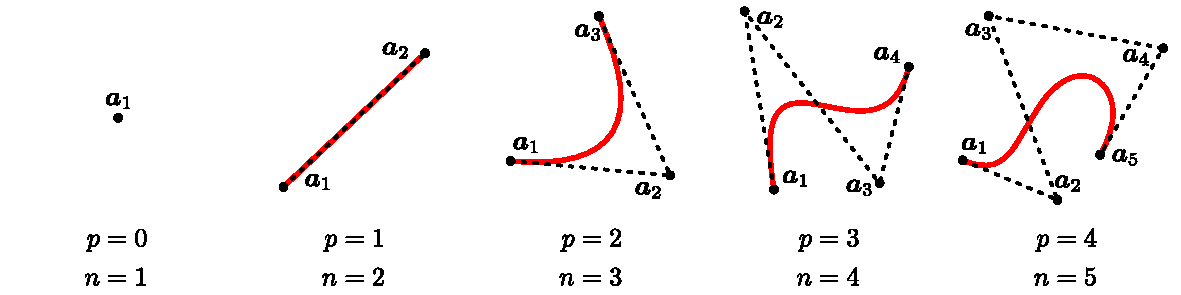
\includegraphics[page=1,clip,width=100mm]{fig.pdf}
	\caption{Bernstein基底関数の例\protect\footnotemark}
	\label{Fig104}
\end{figure}
\footnotetext{\url{https://www.desmos.com/calculator/yc2qe6j6re}}
B\'{e}zier曲線はBernstein基底関数と制御点の線形結合によって定義される.
\begin{screen}
	\begin{defn}
		B\'ezier曲線

		$n$個の点$\bm{a}_1, \dots, \bm{a}_n\in\mathbb{R}^{\tilde{d}}$が与えられたとき, B\'ezier曲線は次式で定義される.
		\begin{align}
			\label{Eqn102}
			\bm{p}:[0,1]\to \setR^{\tilde{d}};t\mapsto \sum_{i=1}^nB_{(i,p)}(t)\bm{a}_i \qquad (p=n-1)
		\end{align}
        ここで$B_{(i,p)}$は$p$次Bernstein基底関数であり, $\bm{a}_i$は制御点と呼ばれる.
	\end{defn}
\end{screen}
次の図\ref{Fig101}に$p\le 4$までのB\'ezier曲線の例を示す.\footnote{(単に定義の問題なのでどちらでも良いのだが)1点しか現れない$p=0$でもB\'{e}zier曲線に含めるとする.}
\newpage

\addtocounter{footnote}{-1}
\begin{figure}[H]
	\centering
    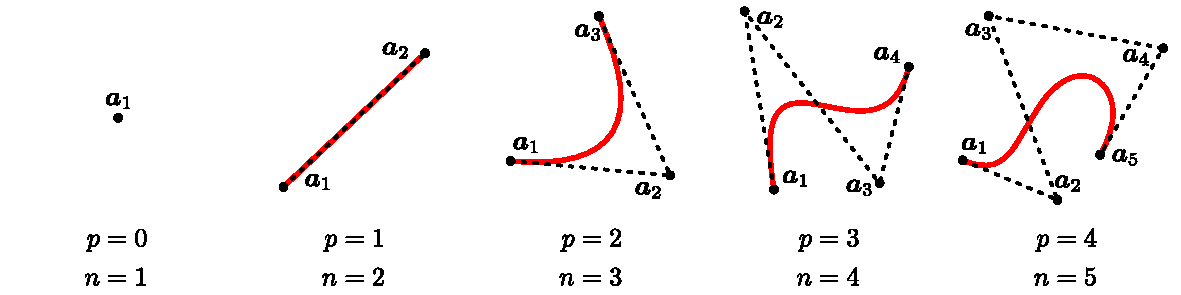
\includegraphics[page=1,clip,width=160mm]{fig.pdf}
    % 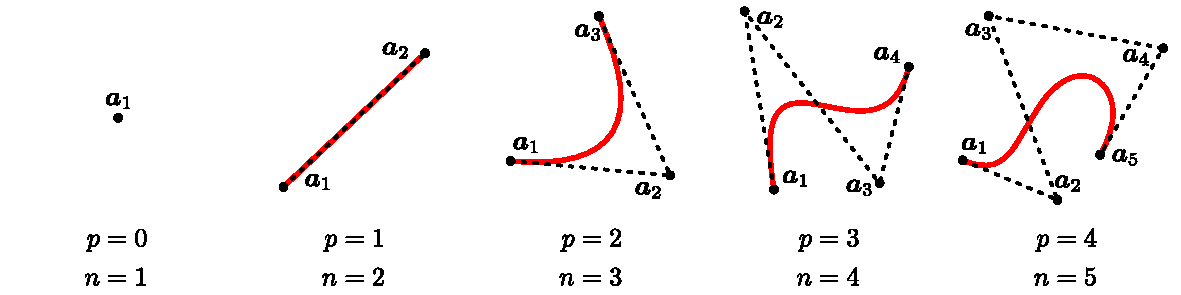
\includegraphics[page=1,clip,width=100mm]{fig.pdf}
	\caption{B\'ezier曲線の例\protect \footnotemark}
	\label{Fig101}
\end{figure}
\footnotetext{\url{https://www.desmos.com/calculator/rkvbtzpipd}}
Bernstein基底関数について次の帰納的な性質が成り立つ.
\begin{screen}
	\begin{thm}
		\label{Thm101}
		Bernstein基底関数の漸化式

        Bernstein基底関数$B_{(i,p)}$について
		\begin{align}
			B_{(i,p)}(t)&=tB_{(i-1,p-1)}(t)+(1-t)B_{(i,p-1)}(t) \\
    		B_{(1,0)}(t)&=1
		\end{align}
		が成立する.
	\end{thm}
\end{screen}
\begin{proof}
    定義に沿って展開して
    \begin{align}
        &\begin{aligned}
            B_{(i,p)}(t)
            &=\nCr{p}{i-1}t^{i-1}(1-t)^{p-i+1} \\
            &=\Pare{\nCr{p-1}{i-2}+\nCr{p-1}{i-1}}t^{i-1}(1-t)^{p-i+1} \\
            % &=\nCr{p-1}{i-2}t^{i-1}(1-t)^{p-i+1}+\nCr{p-1}{i-1}t^{i-1}(1-t)^{p-i+1} \\
            &=t\nCr{p-1}{i-2}t^{i-2}(1-t)^{(p-1)-i+2}+(1-t)\nCr{p-1}{i-1}t^{i-1}(1-t)^{(p-1)-i+1} \\
            &=tB_{(i-1,p-1)}(t)+(1-t)B_{(i,p-1)}(t)
        \end{aligned} \\ \notag \\
        &\begin{aligned}
            B_{(1,0)}(t)
            &=\nCr{0}{1-1}t^{1-1}(1-t)^{0-1+1}
            =1
        \end{aligned}
    \end{align}
    である.
    ただし, $2$項係数の性質から$B_{(0,p)}=B_{(p+2,p)}=0$とした.
\end{proof}

定義\ref{Def101}の代わりに, 定理\ref{Thm101}を以ってBernstein基底関数の定義とする流儀もある.
この流儀は, 後のB-spline基底関数の定義\ref{Def301}で役立つ.
$p\le 3$までの帰納的関係を表したものが次の図\ref{Fig102}である.\footnote{特に主張の無い図に見えるかもしれないが, 後の図\ref{Fig301}と見比べれるのに役立つ.}
\begin{figure}[H]
	\centering
    \includegraphics[page=2,clip,width=80mm]{fig.pdf}
	\caption{Bernstein基底関数の帰納的関係}
	\label{Fig102}
\end{figure}
B\'ezier曲線について次の定理が成り立つ.
\begin{screen}
	\begin{thm}
		\label{Thm105}
		B\'ezier曲線の漸化式 (De Casteljauのアルゴリズム)

        与えられた$n$個の制御点$\bm{a}_i$に対して, $\bm{q}_{(i,j)}(t)$を次の漸化式で定義する.
		\begin{align}
			\bm{q}_{(i,j)}(t)&=t\bm{q}_{(i+1,j-1)}+(1-t)\bm{q}_{(i,j-1)} \\
			\bm{q}_{(i,0)}(t)&=\bm{a}_i
		\end{align}
		このとき, 制御点から構成される$p=n-1$次のB\'{e}zizer曲線$\bm{p}(t)$について
		\begin{align}
			\label{Eqn105}
			\bm{p}(t)=\bm{q}_{(1,p)}(t)
		\end{align}
		が成立する.
	\end{thm}
\end{screen}
\begin{proof}
	写像$\bm{r}_{(i,j)}:[0,1]\to \setR^{\tilde{d}}$を
	\begin{align}
		\bm{r}_{(i,j)}(t)
		=\sum_{k=1}^{j+1} B_{(k,j)}(t)\bm{a}_{k+i-1}
		% \quad (j>0)
	\end{align}
    とおく.
    この$\bm{r}_{(i,j)}$について
    \begin{align}
        &\begin{aligned}
            \bm{r}_{(i,j)}(t)
            &=\sum_{k=1}^{j+1} B_{(k,j)}(t)\bm{a}_{k+i-1} \\
            &=\sum_{k=1}^{j+1} \Pare{tB_{(k-1,j-1)}(t)+(1-t)B_{(k,j-1)}(t)}\bm{a}_{k+i-1} \\
            &=t\sum_{k=1}^{j+1}B_{(k-1,j-1)}(t)\bm{a}_{k+i-1}+(1-t)\sum_{k=1}^{j+1}B_{(k,j-1)}(t)\bm{a}_{k+i-1} \\
            &=t\sum_{k=1}^{j} B_{(k,j-1)}(t)\bm{a}_{k+i}+(1-t)\sum_{k=1}^{j} B_{(k,j-1)}(t)\bm{a}_{k+i-1} \\
            &=t\bm{r}_{(i+1,j-1)}+(1-t)\bm{r}_{(i,j-1)}
        \end{aligned} \\ \notag \\
        &\begin{aligned}
            \bm{r}_{(i,0)}(t)
            &=\sum_{k=1}^{0+1} B_{(k,0)}(t)\bm{a}_{k+i-1} \\
            &=B_{(1,0)}(t)\bm{a}_{1+i-1} \\
            &=\bm{a}_{i}
        \end{aligned}
    \end{align}
    が成り立つから, $\bm{q}_{(i,j)}=\bm{r}_{(i,j)}$である.
    よって
    \begin{align}
        \begin{aligned}
            \bm{q}_{(1,p)}(t)
            =\bm{r}_{(1,p)}(t)
            =\sum_{k=1}^{p+1} B_{(k,p)}(t)\bm{a}_{k+1-1}
            =\sum_{k=1}^{n} B_{(k,p)}(t)\bm{a}_{k}
            =\bm{p}(t)
        \end{aligned}
    \end{align}
    である.
\end{proof}


%\newpage
定理\ref{Thm105}を図で表すと, 例えば$p=3$では図\ref{Fig103}のようになる.
\addtocounter{footnote}{-1}
\begin{figure}[H]
	\centering
    \includegraphics[page=3,clip,width=110mm]{fig.pdf}
	\caption{3次B\'ezier曲線(赤線)\protect\footnotemark}
	\label{Fig103}
\end{figure}
\footnotetext{\url{https://www.desmos.com/calculator/a8kgvjkpkx}}
式(\ref{Eqn102})と式(\ref{Eqn105})が等価であることから, B\'ezier曲線の定義を式(\ref{Eqn105})とする流儀もある.

以降のための準備として, 次に多項式空間を用意する.
\begin{screen}
	\begin{defn}
		多項式空間

		$\mathcal{P}[p]$で$p$次以下の多項式全体を表す.
	\end{defn}
\end{screen}
\begin{screen}
	\begin{thm}
		\label{Thm103}
		多項式空間の線形性

		$\mathcal{P}[p]$には自然に$p+1$次元線形空間としての構造が入り, $p\le q$であれば線形部分空間としての包含関係$\mathcal{P}[p]\subset\mathcal{P}[q]$が成り立つ.
	\end{thm}
\end{screen}
\begin{proof}
    $p$次以下の多項式は$t$を変数として$a_p t^p+a_{p-1} t^{p-1}+\cdots+a_1 t+a_0$の形に書くことができる.
    多項式の線形演算は, 係数$a_i$を取り出せば$\setR^{p+1}$の線形演算と同型であり, よって$\mathcal{P}[p]$には$p+1$次元線形空間の構造が入る.
    包含関係$\mathcal{P}[p]\subset\mathcal{P}[q]$は定義から明らか.
\end{proof}

Bernstein基底関数について以下の定理\ref{Thm106}, \ref{Thm107}が成立する.
\begin{screen}
	\begin{thm}
		\label{Thm106}
		Bernstein基底関数の張る線形空間

		$p$次Bernstein基底関数は$p$次多項式空間$\mathcal{P}[p]$の基底である.
	\end{thm}
\end{screen}
\begin{proof}
	%$\bm{a}_i\in\mathbb{R}^d$であり, 定義において各成分は独立だから, ある1つの成分について調べれば良い.
	%よって$\bm{a}_i$を$a_i\in\mathbb{R}$に置き換え, それについて示せば良い.
	$p$次多項式空間$\mathcal{P}[p]$は$p+1$次元の線形空間であり, $p$次Bernstein基底関数はこの空間の元である.
	基底関数の数は$p+1$個であるから, あとはBernstein基底関数の線形独立性を言えば良い.
	これは$t=0$での微分係数を順に比較することで示される.
\end{proof}
この定理\ref{Thm106}から, 任意の多項式曲線\footnotemark とB\'ezier曲線が等価である事が分かる.
\footnotetext{曲線の各成分が$t$に関する多項式で表される曲線のこと.}
つまり, B\'ezier曲線で放物線は表現できるが, 楕円や双曲線は表現することができない.
次の定理はBernstein基底関数が持つ基本的な性質である.
\begin{screen}
	\begin{thm}
		\label{Thm107}
		1の分割(Bernstein基底関数)

        Bernstein基底関数$B_{(i,p)}$について次が成り立つ.
		\begin{align}
			\sum_{i=1}^{n} B_{(i,p)}(t)= 1, \qquad 0\le B_{(i,p)}(t)\le 1 \qquad(t\in[0,1])
		\end{align}
        ただし$n=p+1$とする.
	\end{thm}
\end{screen}
\begin{proof}\hspace{-0.5em}\footnotemark
	帰納法で示す.
	$
		\displaystyle
		\sum_{i=1}^{p+1} B_{(i,p)}(t)= 1
	$
	は$p=0$については明らかに成立.
	$
		\displaystyle
		\sum_{i=1}^{P} B_{(i,P-1)}(t)= 1
	$
	を仮定すれば
	定理\ref{Thm101}より
	\begin{align}
		\begin{aligned}
            \sum_{i=1}^{P+1} B_{(i,P)}(t)
			&=\sum_{i=1}^{P+1} \Pare{tB_{(i-1,p-1)}(t)+(1-t)B_{(i,p-1)}(t)} \\
			&=t\sum_{i=2}^{P+1}B_{(i-1,p-1)}(t)+(1-t)\sum_{i=1}^{P}B_{(i,p-1)}(t) \\
			&=t+(1-t)
            =1
		\end{aligned}
	\end{align}
	である.
    よって帰納的に任意の$n=p+1$に対して$\sum\limits_{i}B_i(t)=1$が従う.
    Bernstein基底関数の定義と$0\le t\le 1$からすぐに$0\le B_{(i,p)}$が従い, 先の等式を合わせれば$0\le B_{(i,p)}\le 1$が分かる.
\end{proof}
\footnotetext{後の定理\ref{Thm306}と定理\ref{Thm307}を使えば, より一般の場合の別証明が与えられる.}

\newpage
$1$の分割とは, 定数関数$1$を, 幾つかの非負値関数の和に分解する事を意味している.
次の定理\ref{affine}, 定理\ref{convex}は単に$1$の分割から従うものだから, Bernstein基底関数よりも一般的な形で述べる.
\begin{screen}
	\begin{thm}
		\label{affine}
		アフィン不変性\footnotemark

		$1$の分割を充たす基底関数$B_i$とそれに対応する制御点を$\bm{a}_i$とする.
		また, これらから生成される曲線を$\displaystyle\bm{p}(\bm{a}_i;t):=\sum_i B_i(t)\bm{a}_i$で表す.
		このとき, 任意のアフィン変換$T$に対して次が成立する.
		\begin{align}
			T(\bm{p}(\bm{a}_i;t))=\bm{p}(T(\bm{a}_i);t)
		\end{align}
	\end{thm}
\end{screen}
\footnotetext{affine invarianceの訳から習慣的に「アフィン不変性」と呼ばれているが, 「アフィン可換性」とする方が定理をよく表しているように筆者は思う.}
\begin{proof}
	任意のアフィン変換$T$は行列$A$による線形変換とベクトル$\bm{b}$による平行移動の合成で書けるから
	\begin{align}
		\bm{p}(T(\bm{a}_i);t)
		=\sum_iB_i(A\bm{a}_i+\bm{b})
		=A\sum_iB_i\bm{a}_i+\sum_iB_i\bm{b}
		=A\bm{p}(\bm{a}_i;t)+\bm{b}
		=T(\bm{p}(\bm{a}_i;t))
	\end{align}
	である.
\end{proof}
次の図\ref{Fig130}は$5$次B\'{e}zier曲線に対するアフィン不変性の例を示している.
\begin{figure}[H]
	\centering
    \includegraphics[page=13,clip,width=135mm]{fig.pdf}
    % 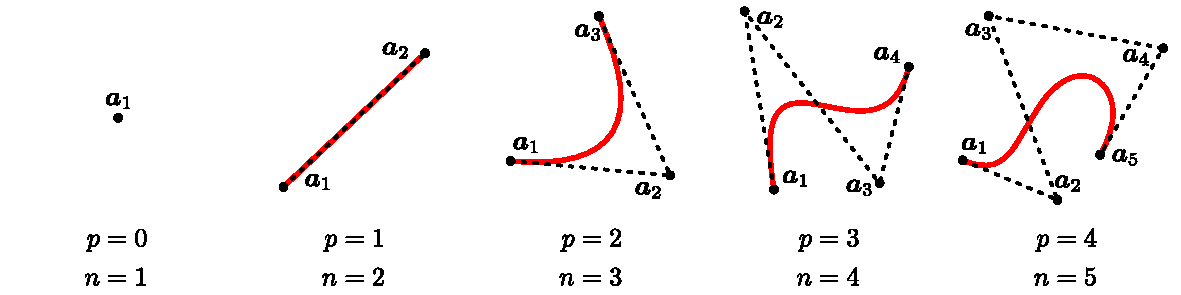
\includegraphics[page=1,clip,width=100mm]{fig.pdf}
	\caption{アフィン不変性の例}
	\label{Fig130}
\end{figure}
アフィン不変性は, 「制御点を平行移動や拡大縮小\footnote{アフィン変換なので, 定理はより一般の変換での成立を主張している.}すれば曲線もそれに追従する」ことを意味しており, これは人間が制御点を直観的に決定することを容易にしている.
次の凸包性に関する性質は, 生成される図形の位置が制御点から見積もれることを主張しており, この性質も人間にとって都合が良い.
\begin{screen}
	\begin{thm}
        \label{convex}
		凸包性

		基底関数$B_i:I\to \setR$, 制御点$\bm{a}_i\in \setR^{\tilde{d}}$から構成される曲線$C$について, 基底関数$B_i$が$1$の分割を充たせば, 曲線$C$は制御点の凸包の部分集合である.
	\end{thm}
\end{screen}
\begin{proof}\hspace{-0.5em}\footnotemark
	制御点の集合$\set{\bm{a}_1,\dots, \bm{a}_n}\subset\setR^{\tilde{d}}$の凸包$\conv_i(\bm{a}_i)$について
	\begin{align}
        \label{Eqn150}
		\conv_i(\bm{a}_i)=\Set{\sum_{i=1}^n c_i\bm{a}_i|\sum_{i=1}^n c_i=1, c_i\in[0,1]}
	\end{align}
	が成り立つ.
	よって$\setR^{\tilde{d}}$の部分集合としての曲線
    \begin{align}
        C=\Set{\sum_i B_i(t)\bm{a}_i | t\in I}
    \end{align}
    と見比べれば$C\subset \conv_i(\bm{a}_i)$が分かる.
\end{proof}
\footnotetext{これは一般的の曲線に対する証明だが, B\'ezier曲線に限れば式(\ref{Eqn150})を経由しない別証明がある:
	\begin{proof}
		定理\ref{Thm105}より$1\leq k\leq n$に対して$\displaystyle\bm{p}_{(i,k)}\in\conv_i(\bm{p}_{(i,k-1)})$であるから
		\begin{align}
			\conv(\bm{p}_{(i,k)})\subset\conv(\bm{p}_{(i,k-1)})
		\end{align}
		である.
		よって帰納的に定理が従う.
	\end{proof}
}
次の図\ref{Fig131}は$5$次B\'{e}zier曲線に対する凸包性の例を示している.
\begin{figure}[H]
	\centering
    \includegraphics[page=14,clip,width=85mm]{fig.pdf}
    % 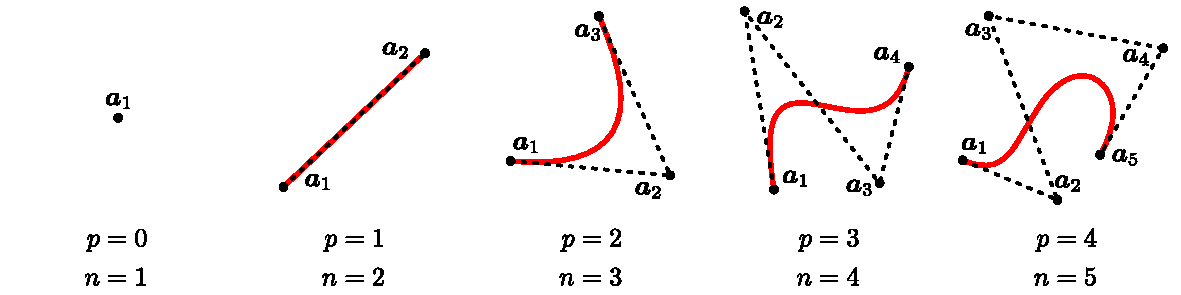
\includegraphics[page=1,clip,width=100mm]{fig.pdf}
	\caption{凸包性の例}
	\label{Fig131}
\end{figure}



\clearpage
% \section{有理曲線}
\section{有理基底関数と有理曲線}
B\'ezier曲線では, 楕円や双曲線を表現できないという問題があった.
これを解決するのが有理基底関数と有理曲線である.
\begin{screen}
	\begin{defn}
		有理基底関数

		$n$個の非負値基底関数$B_i^{(\text{o})}:I\to \setR$とそれに対応する$n$個の実数$w_i$が与えられれば, 有理基底関数は次で定義される.
		\begin{align}
			B_i:I\to \setR;t\mapsto \dfrac{B_{i}^{(\text{o})}(t)w_i}{\sum\limits_{j}B_{j}^{(\text{o})}(t)w_j}
		\end{align}
		ここで$w_i$重みと呼ばれ, 普通は$w_i>0$とする.
        % さらに基底関数について$B_i^{(\text{o})}\le 0$も仮定する.
	\end{defn}
\end{screen}
有理基底関数に対しても次の定理が成立する.
\begin{screen}
	\begin{thm}
		\label{Thm201}
		1の分割 (有理基底関数)

        有理基底関数$B_i$について次が成り立つ.
		\begin{align}
			\sum_i B_i= 1 \qquad
            0\le B_i\le 1
		\end{align}
	\end{thm}
\end{screen}
\begin{proof}
	先の定義を代入して
	\begin{align}
		\sum_i B_i(t)=\sum_i \dfrac{B_{i}^{(\text{o})}(t)w_i}{\sum\limits_{j}B_{j}^{(\text{o})}(t)w_j}= 1
	\end{align}
	である.
	なお, 基底関数$B_i^{(\text{o})}$の$1$の分割$\sum\limits_iB_i^{(\text{o})}= 1$は必ずしも必要ではなかった.
    重みについて$w_i>0$より$B_i\ge 0$が従い, 上の式から$\le 1$でも抑えられる.
\end{proof}
とくに, $B_i^{(\text{o})}$が1の分割を充たし, $w_1=\cdots=w_n$であれば$B_i=B_i^{(\text{o})}$である.
重み$w_i$全体を定数倍しても, 分母分子で約分されるから, 基底関数$B_i$は変わらない.%
\footnote{この意味で定数倍に関して同地関係を取り, 重みを$\setR P^{n-1}$の元として扱える. しかし, $w_i>0$の条件のために$\setR P^{n-1}$全体に対応している訳ではなくあまり利益はない.}
\begin{screen}
	\begin{defn}
		有理曲線

        $n$個の制御点$\bm{a}_1, \dots, \bm{a}_n\in\mathbb{R}^{\tilde{d}}$と有理基底関数$B_i$が与えられれば, 有理曲線は次式で定義される.
		\begin{align}
			\bm{p}(t)=\sum_i B_i(t) \bm{a}_i
		\end{align}
	\end{defn}
\end{screen}
定理\ref{Thm201}より1の分割が充たされるから, 有理曲線もまたアフィン不変性(定理\ref{affine})や凸包性(定理\ref{convex})を充たす.


\newpage
次に, 有理曲線を幾何的に解釈するための定理を与える.
\begin{screen}
	\begin{thm}
		有理曲線と射影の関係

		$\mathbb{R}^{\tilde{d}}$と$\mathbb{R}^{\tilde{d}}\times\{1\}\subset\mathbb{R}^{{\tilde{d}}+1}$を自然な写像で同一視する.
		制御点$\bm{a}_i=(a_i^1,\dots,a_i^{\tilde{d}})\in\mathbb{R}^{\tilde{d}}$に対応する点$(a_i^1,\dots,a_i^{\tilde{d}},1)\in\mathbb{R}^{\tilde{d}}\times\{1\}$を$\bm{a}_i^{({\tilde{d}}+1)}$と書く.
		$\bm{\alpha}_i=w_i \bm{a}_i^{({\tilde{d}}+1)}\in\setR^{\tilde{d}+1}$とおいて, $\mathbb{R}^{{\tilde{d}}+1}$上の曲線$\bm{\pi}(t)=\sum\limits_iB_i^{(\text{o})}(t)\bm{\alpha}_i$を構成する.
		このとき, $\bm{\pi}(t)$を$\mathrm{O}\in\mathbb{R}^{{\tilde{d}}+1}$に関して$\mathbb{R}^{\tilde{d}}\times\{1\}$に射影すれば有理曲線$\bm{p}(t)$が得られる.
	\end{thm}
\end{screen}
\begin{proof}
	射影先の座標を得るには$\bm{\pi}$の第${\tilde{d}}+1$成分でそれ自身を割れば良いから
	\begin{align}
		\bm{p}(t)
		=\frac{\bm{\pi}(t)}{\bm{\pi}(t)\cdot \bm{e}_{\tilde{d}+1}}
		=\frac{\sum\limits_i B_i^{(\text{o})}(t)\bm{\alpha}_i}{\sum\limits_j B_j^{(\text{o})}(t)\bm{\alpha}_j\cdot\bm{e}_{\tilde{d}+1}}
		=\frac{\sum\limits_i B_i^{(\text{o})}(t)w_i\bm{a}_i}{\sum\limits_j B_j^{(\text{o})}(t)w_j}
		=\sum_i {B}_i(t)\bm{a}_i
	\end{align}
	である.
	ここで$\bm{e}_{\tilde{d}+1}=(0,\dots,0,1)\in\mathbb{R}^{\tilde{d}+1}$である.
\end{proof}

% \newpage
この定理を図で表すと次の図\ref{Fig201}のようになる.
\begin{figure}[H]
	\centering
    \includegraphics[page=4,clip,width=120mm]{fig.pdf}
	\caption{曲線の射影}
	\label{Fig201}
\end{figure}
\noindent
$\tilde{d}=2$では可視化するために必要な空間が3次元だから理解しやすいが, $\tilde{d}=3$となると$4$次元空間からの射影が必要となり, 幾何的にイメージするのは少し難しくなる.

\newpage
有理B\'ezier曲線で円弧を表現するには, 図\ref{Fig202}のようにB\'ezier曲線で$\mathbb{R}^3$上の円錐に沿って放物線を作り, それを原点に関して射影すれば良い.%
\footnote{これによって写像$\mathbb{R}\to S^1$が得られるが, この写像は立体射影と本質的に同じパラメータ付けである.}
\addtocounter{footnote}{-1}
\begin{figure}[H]
	\centering
    \includegraphics[page=5,clip,width=160mm]{fig.pdf}
	\caption{有理B\'ezier曲線による円弧の表現\protect \footnotemark}
	\label{Fig202}
\end{figure}
\footnotetext{\url{https://www.desmos.com/calculator/92allkrzw7}}

もっとも, 有理基底関数はB\'ezier曲線を円弧などに拡張するためだけのものではない.
次の定理は係数$w_i$が重みと呼ばれる理由を与える.
\begin{screen}
	\begin{thm}
		重みの極限

		基底関数$B_i^{\text{(o)}}:I\to\setR$と重み$w_i$から生成される有理基底関数を$B_i$とする.
        このとき, 任意の$j\in\Z{1}{n}, t\in I$に対して, $B_{j}^{(\text{o})}(t)\neq 0$であれば
		\begin{align}
			B_i(t)\to
			\begin{cases}
				1 &(i=j) \\
				0 &(i\neq j)
			\end{cases} \qquad
            \Pare{\max\Pare{\frac{w_0}{w_{j}},\dots,\frac{w_{{j}-1}}{w_{j}},\frac{w_{{j}+1}}{w_{j}},\dots,\frac{w_n}{w_{j}}}
			\to
			0}
		\end{align}
		が成り立つ.
	\end{thm}
\end{screen}
\begin{proof}
	$i\neq j$について
	\begin{align}
		B_i(t)
		=
		\dfrac{B_{i}^{(\text{o})}(t)w_i}{\sum\limits_{k}B_{k}^{(\text{o})}(t)w_k}
		=
		\dfrac{B_{i}^{(\text{o})}(t)\frac{w_i}{w_{j}}}{\sum\limits_{k}B_{k}^{(\text{o})}(t)\frac{w_k}{w_{j}}}
		\to
		0
	\end{align}
	である.
	さらに1の分割(定理\ref{Thm201})より$i=j$について
	% \begin{align}
	% 	B_i(t)
	% 	\to
	% 	1
	% \end{align}
	$B_i(t)\to 1$
    である.
\end{proof}
\newpage
この定理の例として$5$次有理Bernstein基底関数を考えれば, 次の図\ref{Fig212}のようになる.
ここで, 簡単のために$w_1=w_2=w_4=w_5=w_6=1$とし, $w_3$をパラメータとした.
図中の色付きの曲線が有理Bernstein基底関数$B_3$である.
\addtocounter{footnote}{-1}
\begin{figure}[H]
	\centering
    \includegraphics[page=6,clip,width=160mm]{fig.pdf}
	\caption{有理Bernstein基底関数\protect \footnotemark}
	\label{Fig212}
\end{figure}
\footnotetext{\url{https://www.desmos.com/calculator/czb6vigneh}}

\noindent
図\ref{Fig212}に示したこれらの基底関数から生成される有理B\'ezier曲線は, それぞれ次の図\ref{Fig213}のような曲線を描く.
\addtocounter{footnote}{-1}
\begin{figure}[H]
	\centering
    \includegraphics[page=7,clip,width=130mm]{fig.pdf}
	\caption{有理B\'ezier曲線 \protect\footnotemark}
	\label{Fig213}
\end{figure}
\footnotetext{\url{https://www.desmos.com/calculator/lojzonnjop}}


\clearpage
% \section{B-spline曲線}
\section{B-spline基底関数とB-spline曲線}
B\'ezier曲線では($C^\omega$級\footnotemark の)多項式曲線しか表せなかった.
\footnotetext{ある関数$f$が$C^\omega$級であるとは定義域上の任意の点でのTaylor展開が収束し, その点の近傍で一致するものをいう.
定義より明らかに$C^\infty\subset C^\omega$である.
$f$が$C^\omega$級であれば局所的性質から大域的性質まで決まってしまう.
曲がりパイプなど, 実用的な形状の多くは$C^\omega$級ではない.}
一般に, ある曲線を1つの低次B\'ezier曲線のみで近似することは困難であるため, 近似精度を良くするには複数のB\'ezier曲線を繋げる必要がある.
出来るだけ滑らかに多項式曲線$(=\text{B\'ezier曲線})$を区分的に繋げたものが, 本節で扱うB-spline曲線である.
B\'ezier曲線, 有理曲線と同じように, 制御点$\bm{a}_i$に対応するB-spline基底関数$B_{(i,p)}$を$1$の分割が充たされるように作る.
これまでと大きく異なる点は, 区分点の情報を入れるために広義単調増加な実数の有限列$\bm{k}=(k_1, \dots , k_l)$を用意する所にある.
ここで$\bm{k}$はノット列%
\footnote{英語ではknot vectorと呼ばれるが, $\bm{k}$に対して(単位元や逆元の存在する通常の)加法やスカラー倍を定義する訳ではないから, 単にノット列とする方が筆者の好みである.
}, $k_{i}$はノットと呼ばれる.
%ノットは$t$の動く範囲に対応した数である.
つまり, ある区間$[k_{i}, k_{i+1})$に一つの多項式曲線が対応し, 別の区間$[k_{j}, k_{j+1})$には別の多項式曲線が対応するようにするのである.%
\footnote{多項式の繋ぎ目にあたる数が$k_{i}$になっており, これがノット(knot)と呼ばれる理由である.}
定義$\ref{Def101}$のように, B-spline基底関数$B_{(i,p)}$を直接定義することも可能ではあるが, あまりにも天下り的で, $2$項係数に対応する部分が複雑になってしまう.
それを避けるため, B-spline基底関数では定理\ref{Thm101}のような, 漸化式を以って定義とすることが通常である.
これが次の定義\ref{Def301}である.
\begin{screen}
	\begin{defn}
        \label{Def301}
		B-spline基底関数 (Cox-de Boorの漸化式)

		与えられたノット列$\bm{k}=(k_1, \dots , k_l)$に対するB-spline基底関数は次式で定義される:
		\begin{align}
			\label{Eqn301}
			&{B}_{(i,p)}(t)
			=
			\frac{t-k_{i}}{k_{i+p}-k_{i}}{B}_{(i,p-1)}(t)
			+\frac{k_{i+p+1}-t}{k_{i+p+1}-k_{i+1}}{B}_{(i+1,p-1)}(t), \\
			%
			\label{Eqn302}
			&{B}_{(i,0)} (t)
			=
			\begin{cases}
				&1\quad (k_{i}\le t< k_{i+1})\\
				&0\quad (\text{otherwise})
			\end{cases}
		\end{align}
		ただし, 式(\ref{Eqn301})において分母が$0$であればその項を$0$とする.
	\end{defn}
\end{screen}
次の図\ref{Fig301}は$n=7$とした際の$p\leq 3$までの基底関数の漸化式による定義の関係を表したものである.
\begin{figure}[H]
	\centering
    \includegraphics[page=8,clip,width=75mm]{fig.pdf}
	\caption{B-Spline基底関数の漸化式による定義}
	\label{Fig301}
\end{figure}
\noindent
% 定義式\eqref{Eqn301}の右辺の$B_{(i,p-1)},B_{(i+1,p-1)}$の係数は, それぞれ区間$\supp(B_{(i,p-1)}), \supp(B_{(i+1,p-1)})$\footnotemark 上での1次関数であり, この区間上で$0$から$1$まで(或いは$1$から$0$まで)変化する.
定義式\eqref{Eqn301}の右辺の$B_{(i,p-1)},B_{(i+1,p-1)}$の係数は, それぞれ区間$\squa{k_{i},k_{i+p}}=\supp(B_{(i,p-1)}), \squa{k_{i+1},k_{i+p+1}}=\supp(B_{(i+1,p-1)})$上(定理\ref{Thm301}参照)での1次関数であり, この区間上で$0$から$1$まで(或いは$1$から$0$まで)変化する.
% \footnotetext{ある関数$f:S\to \setR$に対して$\supp(f)\subset S$を$f$の台といい, $\supp(f)=\overline{\set{x\mid f(x)\neq 0}}$で定義される.}
$p\leq 3$までの基底関数$B_{(i,p)}$は例えば次の図\ref{Fig302}のようになる.
\addtocounter{footnote}{-1}
\begin{figure}[H]
	\centering
    % \includegraphics[page=9,clip,width=115mm]{fig.pdf}
    \includegraphics[page=9,clip,width=111mm]{fig.pdf}
	\caption{B-Spline基底関数の例\protect\footnotemark}
	\label{Fig302}
\end{figure}
\footnotetext{\url{https://www.desmos.com/calculator/ql6jqgdabs}}

\newpage
次の定理はB-spline基底関数の性質の中でも特に基本的である.
\begin{screen}
	\begin{thm}
		\label{Thm301}
		B-spline基底関数の台

		ノット列$\bm{k}=(k_1,\dots,k_l)$から生成されるB-spline基底関数$B_{(i,p)}$について
		\begin{align}
			\supp(B_{(i,p)})=\Cl{(k_{i}, k_{i+p+1})}
		\end{align}
		が成り立つ.
	\end{thm}
\end{screen}
\begin{proof}
    $k_{i}=k_{i+p+1}$であれば明らかなので, 以降では$k_{i}\neq k_{i+p+1}$を仮定する.
	B-spline基底関数の定義式(\ref{Eqn301}), (\ref{Eqn302}) (及び図\ref{Fig301})より, $t\not\in[k_{i}, k_{i+p+1}]$において$B_{(i,p)}(t)=0$である.
	よって
	\begin{align}
		\supp(B_{(i,p)})\subset[k_{i}, k_{i+p+1}]
	\end{align}
	である.
	更にB-spline基底関数の定義より, $k_l\neq k_{l+1} \ (l=i,\dots,i+p)$であれば各開区間$(k_{l}, k_{l+1})$においては$B_{(i,p)}> 0$あり, $\supp(B_{(i,p)})\supset[k_l, k_{l+1}]$である.
	よって$k_{i}\neq k_{i+p+1}$であれば
	\begin{align}
		\supp(B_{(i,p)})
        \supset\bigcup_{j\in \Z{i}{i+p}, \ k_{j}\neq k_{j+1}}[k_{j}, k_{j+1}]=[k_{i}, k_{i+p+1}]
	\end{align}
	である.
	よって
	\begin{align}
		\supp(B_{(i,p)})=[k_{i}, k_{i+p+1}]=\Cl{(k_{i}, k_{i+p+1})}
	\end{align}
	である.
\end{proof}

次の定理はノットの配置がB-spline基底関数の決定に及ぼす影響を述べる.
\begin{screen}
	\begin{thm}
		\label{Thm302}
		B-spline基底関数のノット依存性

		$p\ge 1$に対し, $B_{(i,p)}|_{[k_j,k_{j+1}]}$はノット列の部分列$ \pare{k_{j-p+1}, \dots ,k_{j+p}} $のみによって決定される.
	\end{thm}
\end{screen}
\begin{proof}
    帰納法で示す.
    $p=1$については明らか.
    % 帰納法で示す.
    $t\in [k_{j},k_{j+1}]$とする.
    B-spline基底関数の定義式\eqref{Eqn301}において, 係数の$\frac{t-k_{i}}{k_{i+p}-k_{i}},\frac{k_{i+p+1}-t}{k_{i+p+1}-k_{i+1}}$が影響するのはそれぞれ$t\in \supp(B_{(i,p-1)})=\Cl{(k_{i},k_{i+p})}, t\in \supp(B_{(i+1,p-1)})=\Cl{(k_{i+1},k_{i+p+1})}$の場合である.
    よって帰納的に$B_{(i,p)}(t)$は$k_{j-p+1},\dots,k_{j+p}$のみで決定され, 定理が従う.
\end{proof}
次の図\ref{Fig303}は$p=3$での例である.
\addtocounter{footnote}{-1}
\begin{figure}[H]
	\centering
    % \includegraphics[page=9,clip,width=115mm]{fig.pdf}
    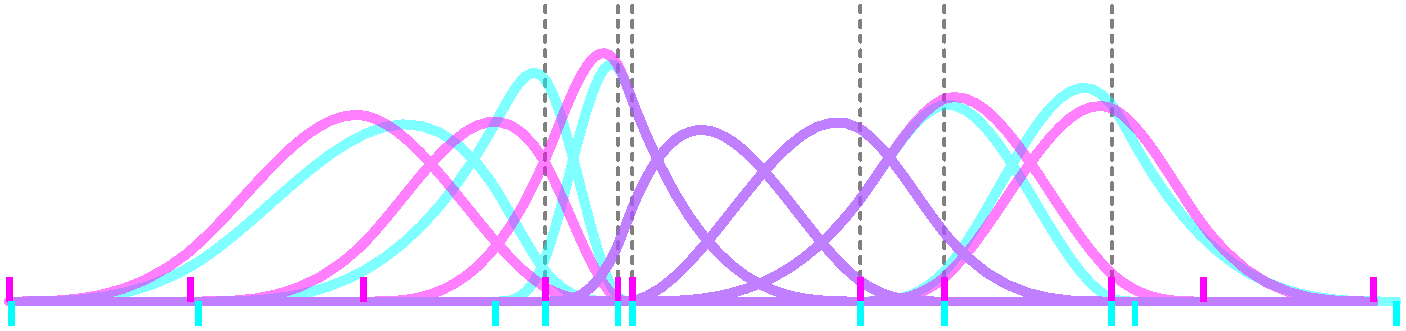
\includegraphics[page=1,clip,width=150mm]{figA.pdf}
	\caption{B-Spline基底関数を決定するノット列\protect\footnotemark}
	\label{Fig303}
\end{figure}
\footnotetext{\url{https://www.desmos.com/calculator/wnp8e4xyyj}}


\newpage
\begin{screen}
	\begin{thm}
		\label{Thm303}
		B-spline基底関数を決定するノット列

		$B_{(i,p)}|_{[k_{i+j},k_{i+j+1}]}$はノット列の部分列
		\begin{align}
			\begin{cases}
				\pare{k_{i}, \dots ,k_{i+p}} \quad & (j=0) \\
				\pare{k_{i}, \dots ,k_{i+p+1}} \quad & (j\in\Z{1}{p-1}) \\
				\pare{k_{i+1}, \dots ,k_{i+p+1}} \quad & (j=p)
			\end{cases}
		\end{align}によって決定される.
	\end{thm}
\end{screen}
\begin{proof}
	定理\ref{Thm301}と定理\ref{Thm302}を合わせれば明らか.
\end{proof}
B-spline基底関数の導関数に対しても, 定義式と同様に漸化式が存在する.
\begin{screen}
	\begin{thm}
		\label{Thm304}
		B-spline基底関数の導関数

        B-spline基底関数$B_{(i,p)}$の導関数$\dot{B}_{(i,p)}$について次が成り立つ.
		\begin{align}
			\label{Eqn304}
			\dot{B}_{(i,p)}(t)=p\Pare{\frac{1}{k_{i+p}-k_{i}}B_{(i,p-1)}(t)-\frac{1}{k_{i+p+1}-k_{i+1}}B_{(i+1,p-1)}(t)}
		\end{align}
		ただし$t\in[k_1, k_l]\backslash \{k_1,\dots,k_l\}$とするが, $t=k_j$において$B_{(i,p-1)}(t), B_{(i+1,p-1)}(t)$が連続であれば, $t$の範囲を$k_j$の近傍までも含める事ができる.
		右辺各項において分母が$0$となる場合は, 定義\ref{Def301}と同様にその項を無視した形の式が成立する.
	\end{thm}
\end{screen}
\begin{proof}
	帰納法で証明する.
	\begin{align}
		&\mathcal{B}_p=\frac{1}{k_{i+p}-k_{i}}B_{(i,p-1)}-\frac{1}{k_{i+p+1}-k_{i+1}}B_{(i+1,p-1)}, \\
		&I=[k_1, k_l]\backslash \{k_1,\dots,k_l\}
	\end{align}
	とおく.
	$B_{(i,0)}$が区分的定数だから$I$上で$\dot{B}_{(i,0)}=0$であり
	\begin{align}
		\begin{aligned}
			\dot{B}_{(i,1)}&=
			\frac{1}{k_{i+1}-k_{i}}B_{(i,0)}-\frac{1}{k_{i+1+1}-k_{i+1}}B_{(i+1,0)}
			+\frac{t-k_{i}}{k_{i+1}-k_{i}}\dot{B}_{(i,0)}+\frac{k_{i+1+1}-t}{k_{i+1+1}-k_{i+1}}\dot{B}_{(i+1,0)} \\
			&=\mathcal{B}_1+0+0
			=1\mathcal{B}_1
		\end{aligned}
	\end{align}
	である.
	よって$p=1$について式(\ref{Eqn304})が成立する.
	続いて
	$p=P-1$で式(\ref{Eqn304})が成立すると仮定すれば
	\begin{align}
		\begin{aligned}
			\dot{B}_{(i,P)}&=
			\frac{1}{k_{i+P}-k_{i}}B_{(i,P-1)}-\frac{1}{k_{i+P+1}-k_{i+1}}B_{(i+1,P-1)} \\
			&\qquad+\frac{t-k_{i}}{k_{i+P}-k_{i}}\dot{B}_{(i,P-1)}+\frac{k_{i+P+1}-t}{k_{i+P+1}-k_{i+1}}\dot{B}_{(i+1,P-1)} \\
			&=\mathcal{B}_P+\frac{t-k_{i}}{k_{i+P}-k_{i}}(P-1)\Pare{\frac{1}{k_{i+P-1}-k_{i}}B_{(i,P-2)}-\frac{1}{k_{i+P}-k_{i+1}}B_{(i+1,P-2)}} \\
			&\qquad+\frac{k_{i+P+1}-t}{k_{i+P+1}-k_{i+1}}(P-1)\Pare{\frac{1}{k_{i+P}-k_{i+1}}B_{(i+1,P-2)}-\frac{1}{k_{i+P+1}-k_{i+2}}B_{(i+2,P-2)}}
		\end{aligned}
	\end{align}
	である.
	ここで記号の見やすさのために$a=k_{i}, b=k_{i+1}, c=k_{i+2}, A=k_{i+P-1}, B=k_{i+P}, C=k_{i+P+1}$とおくと
	\footnote{$B$がB-spline基底関数$B_{(i,p)}$と紛らわしいかもしれないが, 実際には問題にならない.}

	\begin{align}
		\label{Eqn383}
		\begin{aligned}
			\dot{B}_{(i,P)}
			&=\mathcal{B}_P
			+(P-1)
			\left(
			\frac{t-a}{B-a}\Pare{\frac{1}{A-a}B_{(i,P-2)}-\frac{1}{B-b}B_{(i+1,P-2)}}
			\right. \\
			&\hspace{8em}\left.
			+\frac{C-t}{C-b}\Pare{\frac{1}{B-b}B_{(i+1,P-2)}-\frac{1}{C-c}B_{(i+2,P-2)}}
			\right)
		\end{aligned}
	\end{align}
	である.
	ここで
	\begin{align}
		\label{Eqn384}
		\begin{aligned}
			\mathcal{B}_P
			&=\frac{1}{k_{i+P}-k_{i}}B_{(i,P-1)}-\frac{1}{k_{i+P+1}-k_{i+1}}B_{(i+1,P-1)} \\
			&=\frac{1}{k_{i+P}-k_{i}}\Pare{\frac{t-k_{i}}{k_{i+P-1}-k_{i}}B_{(i,P-2)}+\frac{k_{i+P}-t}{k_{i+P}-k_{i+1}}B_{(i+1,P-2)}} \\
			&\qquad-\frac{1}{k_{i+P+1}-k_{i+1}}\Pare{\frac{t-k_{i+1}}{k_{i+P}-k_{i+1}}B_{(i+1,P-2)}+\frac{k_{i+P+1}-t}{k_{i+P+1}-k_{i+2}}B_{(i+2,P-2)}} \\
			&=\frac{1}{B-a}\Pare{\frac{t-a}{A-a}B_{(i,P-2)}+\frac{B-t}{B-b}B_{(i+1,P-2)}} \\
			&\qquad-\frac{1}{C-b}\Pare{\frac{t-b}{B-b}B_{(i+1,P-2)}+\frac{C-t}{C-c}B_{(i+2,P-2)}} \\
			&=\frac{1}{B-a}\Pare{\frac{t-a}{A-a}B_{(i,P-2)}+\frac{B-t}{B-b}B_{(i+1,P-2)}} \\
			&\qquad-\frac{1}{C-b}\Pare{\frac{t-b}{B-b}B_{(i+1,P-2)}+\frac{C-t}{C-c}B_{(i+2,P-2)}} \\
			&\hspace{7em}\quad-\frac{t-a}{B-a}\Pare{\frac{1}{A-a}B_{(i,P-2)}-\frac{1}{B-b}B_{(i+1,P-2)}} \\
			&\hspace{7em}\qquad-\frac{C-t}{C-b}\Pare{\frac{1}{B-b}B_{(i+1,P-2)}-\frac{1}{C-c}B_{(i+2,P-2)}} \\
			&\hspace{7em}\quad+\frac{t-a}{B-a}\Pare{\frac{1}{A-a}B_{(i,P-2)}-\frac{1}{B-b}B_{(i+1,P-2)}} \\
			&\hspace{7em}\qquad+\frac{C-t}{C-b}\Pare{\frac{1}{B-b}B_{(i+1,P-2)}-\frac{1}{C-c}B_{(i+2,P-2)}} \\
			&=\Pare{\frac{B-t}{B-a}-\frac{t-b}{C-b}+\frac{t-a}{B-a}-\frac{C-t}{C-b}}\frac{B_{(i+1,P-2)}}{B-b} \\
			&\hspace{7em}\quad+\frac{t-a}{B-a}\Pare{\frac{1}{A-a}B_{(i,P-2)}-\frac{1}{B-b}B_{(i+1,P-2)}} \\
			&\hspace{7em}\qquad+\frac{C-t}{C-b}\Pare{\frac{1}{B-b}B_{(i+1,P-2)}-\frac{1}{C-c}B_{(i+2,P-2)}} \\
		\end{aligned}
	\end{align}
	であり
	\begin{align}
		\label{Eqn385}
		\begin{aligned}
			\frac{B-t}{B-a}-\frac{t-b}{C-b}+\frac{t-a}{B-a}-\frac{C-t}{C-b}
			&=\frac{B}{B-a}+\frac{b}{C-b}-\frac{a}{B-a}-\frac{C}{C-b} \\
			&=\frac{B(C-b)+b(B-a)-a(C-b)-C(B-a)}{(B-a)(C-b)}=0
		\end{aligned}
	\end{align}
	である.
	したがって以上の式(\ref{Eqn383})(\ref{Eqn384})(\ref{Eqn385})を合わせて
	\begin{align}
		\dot{B}_{(i,P)}=\mathcal{B}_P+(P-1)\mathcal{B}_P=P\mathcal{B}_P
	\end{align}
	を得る.
	よって帰納的に任意の${p}\in[1,l-2]_\setZ, \ {t} \in I$に対して式(\ref{Eqn304})が成立する.
	さらに$B_{(i,p-1)}, B_{(i+1,p-1)}$が$k_j$の近傍で連続であれば$k_j$の近傍でも式(\ref{Eqn304})が成立する.
	これは$B_{(i,p)}$が$k_j$の近傍で連続であり, 導関数が$t\to k_j$で収束するためである.%
	\footnote{これは次の補題から従う.
	\begin{lem*}
	    $f\in C(I,\mathbb{R})$が$I\backslash \{a\}$で微分可能で$\displaystyle\lim_{x\to a} f'(x)$が存在すれば$f$は$a$において微分可能で
	    $\displaystyle f'(a)=\lim_{x\to a}f'(x)$が成立する.
	\end{lem*}
	\begin{proof}
	    定数$c$と関数$g$を
	    \begin{align}
	        c:=\lim_{x\to a}f'(x),\quad
	        g(x):=f(x+a)-f(a)-cx
	    \end{align}
	    とおくと
	    $
	        \displaystyle
	        g(0)=0,\
	        g'(x)=f'(x+a)-c,\
	        \lim_{x \to 0} g'(x)=0
	    $
	    である.
	    よってあとは
	    \begin{align}
	        g'(0)=0
	    \end{align}
	    を示せば良い.
	    $\displaystyle \lim_{x\to 0}g'(x)=0$を$\varepsilon$-$\delta$で表せば
	    \begin{align}
	        \A \varepsilon>0, \E \delta>0 \ ; \ |x|<\delta\Rightarrow |g'(x)|<\varepsilon
	    \end{align}
	    である.
	    $0<x_0<\delta$なる$x_0$において$g(x_0)>\varepsilon x_0$を仮定する.
	    $d:=g(x_0)-\varepsilon x_0>0$とおく.
	    このとき微積分学の基本定理より
	    \begin{align}
	        g(x)=\int_{x_0}^x g'(x) dx+g(x_0)>\varepsilon (x-x_0)+\varepsilon x_0 +d=\varepsilon x +d
	    \end{align}
	    である.
	    よって$\displaystyle \lim_{x\to 0}g(x)\geq d>0=g(0)$
	    よりこれは$g$の連続性に矛盾.
	    したがって$g(x_0)\leq\varepsilon x_0$である.
	    同様にして$|x_0|<\delta\Rightarrow |g(x_0)|\leq \varepsilon |x_0|$である.
	    よって
	    \begin{align}
			\A \varepsilon>0, \
			\E \delta>0\
			;\
			|x_0|<\delta
			\Rightarrow
	        g'(0)=\Abs{\frac{g(x_0)-g(0)}{x_0}}\leq\varepsilon
	    \end{align}
	    であり, $g'(0)=0$である.
	\end{proof}
	}
	$k_{i+p}-k_{i}=0$または$k_{i+p+1}-k_{i+1}=0$なる場合も同様の議論から示される.
\end{proof}

後の定理のために, ノット列の重複度を返す関数を用意する.

\begin{screen}
	\begin{defn}
	     ノット列の重複に関する記号

         ノット列$\bm{k}=(k_1,\dots,k_l)$, 次数$p\in \setN$に対して, 関数$\N_{(i,p)}:\setR\to \setN, \N:\setR\to \setN$を次で定義する.
         \begin{align}
             \N_{(i,p)}(t)
             &=\#\Set{j\in\Z{i}{i+p+1}|k_j=t} \\
             \N(t)
             &=\#\Set{j\in\Z{1}{l}|k_j=t}
         \end{align}
	\end{defn}
\end{screen}
B-spline基底関数$B_{(i,p)}$に影響を与えるノット列の重複を返す関数が$\N_{(i,p)}$である.
それに対して$\N$は単にノットの重複を返す関数であり, とくに基底関数を選ぶ訳ではない.
明らかに$\N_{(i,p)}(t)\le \N(t)$であり, $\N(t)\neq 0$であれば$t\in\Set{k_1,\dots, k_l}$である.
$\N_{(i,p)}$は直ぐ後の定理\ref{Thm305}で, $\N$はもう少し後の定義\ref{Def305}で使うことになる.

\begin{screen}
	\begin{thm}
		\label{Thm305}
		B-spline基底関数の微分可能性

        B-spline基底関数$B_{(i,p)}$について, 次の性質が成り立つ.
        \begin{enumerate}
			\renewcommand{\labelenumi}{(\roman{enumi})}
			\item ノット列$\bm{k}$に重複が無ければ, 基底関数は$B_{(i,p)}\in C^{p-1}(\setR)$なる区分$p$次多項式である.
			\item
            \begin{itemize}
                \item $p-\N_{(i,p)}(t^*)=-2$なる$t^*$が存在すれば$B_{(i,p)}= 0$.
                \item $p-\N_{(i,p)}(t^*)=-1$ならば$B_{(i,p)}$は$t^*$で不連続.
                \item $p-\N_{(i,p)}(t^*)\ge 0$ならば$B_{(i,p)}$は$t^*$の近傍において$C^{p-\N_{(i,p)}(t^*)}$級である.
            \end{itemize}
		\end{enumerate}
	\end{thm}
\end{screen}
\newpage
\begin{proof}
    \begin{enumerate}
        \renewcommand{\labelenumi}{(\roman{enumi})}
        \item 帰納法で証明する.
    	ノットに重複が無ければ$B_{(i,1)}$は連続だから$C^0$級.
    	よって$p=1$について成立.
    	$p=P-1$で$B_{(i,p)}$が$C^{p-1}=C^{P-2}$級であれば, 定理\ref{Thm304}より$B_{(i,P)}$の導関数が$C^{P-2}$級となる.
    	よって$B_{(i,P)}$は$C^{P-1}$級である.
    	したがって帰納的に定理が成立する.
        \item
        \begin{itemize}
            \item $p-\N_{(i,p)}(t^*)=-2$なる$t^*$が存在すれば, 基底関数の定義式(\ref{Eqn301}), (\ref{Eqn302})より基底関数を構成するノットは全て等しい.
            よって帰納的に$B_{(l,p)}= 0$.

            \item $p-\N_{(i,p)}(t^*)=-1$なる場合について, $k_{i}<k_{i+1}=\dots=k_{i+p+1}=t^*$または$t^*=k_{i}=\dots=k_{i+p}<k_{i+p+1}$である.
            $k_{i}<k_{i+1}=\dots=k_{i+p+1}=t^*$では基底関数の定義式(\ref{Eqn301}), (\ref{Eqn302})より
            %\newpage
            \begin{align}
                B_{(i,p)}(t)=
                \begin{cases}
                    \Pare{\dfrac{t-k_{i}}{k_{i+p+1}-k_{i}}}^p &(t\in[k_{i}, k_{i+p+1}))\\
                    0 &(\text{otherwise})
                \end{cases}
            \end{align}
            である.
            よって$B_{(l,p)}$は$t^*$で不連続である.
            $t^*=k_{i}=\dots=k_{i+p}<k_{i+p+1}$の場合でも同様である.

            \item $p-\N_{(i,p)}(t^*)\ge 0$なる場合について.
            $t^*=k_j=\cdots=k_{j+\N_{(i,p)}(t^*)-1}$を充たす$j\in[i,i+p+1]_\setZ$が存在.
            よって, 上に見たように$B_{(j,\N_{(i,p)}(t^*)-2)}=0$である.
            同様に上に見たように, $\tilde{i}\in [i, i+p-\N_{(i,p)}(t^*)+1]_\setZ$に対して$B_{(\tilde{i},\N_{(i,p)}(t^*)-1)}$は$t^*$で不連続である.
            したがって, $\tilde{i}\in [i, i+p-\N_{(i,p)}(t^*)]_\setZ$に対して$B_{(\tilde{i},\N_{(i,p)}(t^*))}$は$t^*$で連続($C^0$級)である.
            よって, 定理\ref{Thm304}より帰納的に$\tilde{i}\in [i, i+p-\N_{(i,p)}(t^*)-r]_\setZ$に対して$B_{(\tilde{i},\N_{(i,p)}(t^*)+r)}$は$t^*$の近傍で$C^r$級である.
            ゆえに, $r=p-\N_{(i,p)}(t^*)$を考えれば$B_{(i,p)}$は$t^*$の近傍で$C^{p-\N_{(i,p)}(t^*)}$級である.\footnotemark
        \end{itemize}
    \end{enumerate}
    ここで, (ii)の3番目は(i)を特別な場合として含んでいることに注意.
\end{proof}
\footnotetext{証明の文章だけでは分かり難いため, 適宜図\ref{Fig301}を参照されたい.}

\begin{screen}
	\begin{thm}
        \label{Thm313}
        基底関数の極大点一意性

        B-spline基底関数$B_{(i,p)}$のそれぞれに対して$\tau_{(i,p)}\in \setR$が存在し, $B_{(i,p)}$は$(-\infty, \tau_{(i,p)})$で広義単調増加, $[\tau_{(i,p)},+\infty)$で広義単調減少となる.
        とくに, $B_{(i,p)}\in C^0(\setR)$なら$[k_{i},\tau_{(i,p)}]$で狭義単調増加, $[\tau_{(i,p)}, k_{i+p+1}]$で狭義単調減少とできる.
	\end{thm}
\end{screen}
\begin{proof}
    $p=0$に対しては$\tau_{(i,p)}=k_{i+1}$, $p=1$に対しても$\tau_{(i,p)}=k_{i+1}$とすれば良い.
    $p-\N_{(i,p)}(t^*)=2$なる$t^*$が存在すれば, $B_{(i,p)}$は定数0だから$\tau_{(i,p)}$は任意に取れる.
    $p-\N_{(i,p)}(t^*)=1$なる$t^*$が存在すれば, $k_{i}<k_{i+1}=\cdots=k_{l-1}<k_{l}$であって, $t^*=k_{i+1}, B_{(i,p)}(t^*)=1$であるから, $\tau_{(i,p)}=k_{i+1}$とすれば良い.

    よって以降では, $p\ge 2$, $B_{(i,p)}\in C^1(\setR)$と仮定して良い.
    この場合に, より強く
    \begin{align}
        \label{Eqn303}
        \exists \tau_{(i,p)}\in \supp(B_{(i,p)}) \ \text{s.t.} \ B_{(i,p)}|_{\squa{k_{i}, \tau_{(i,p)}}}, -B_{(i,p)}|_{\squa{\tau_{(i,p)},k_{i+p+1}}}は狭義単調増加
    \end{align}
    が成り立つことを以下で示す.

    関数$C_{(i,p)}$を次で定義する.\footnote{$k_{i+p+1}-k_i=0$であれば$B_{(i,p)}=0$であった. しかし, $C_{(i,p)}$は(定数倍の差はあるが)Diracの$\delta$関数のように定義する方が自然である.}
    \begin{align}
        C_{(i,p)}
        =\frac{1}{k_{i+p+1}-k_{i}}B_{(i,p)}
    \end{align}
    ここで次が成り立つ.
    \begin{align}
        B_{(i,p)}&=(t-k_{i})C_{(i,p-1)}+(k_{i+p+1}-t)C_{(i+1,p-1)} \\
        \dot{B}_{(i,p)}&=p(C_{(i,p-1)}-C_{(i+1,p-1)}) \\
        \label{Eqn307}
        C_{(i,p)}&=\frac{t-k_{i}}{k_{i+p+1}-k_{i}}C_{(i,p-1)}+\frac{k_{i+p+1}-t}{k_{i+p+1}-k_{i}}C_{(i+1,p-1)} \\
        \label{Eqn308}
        \dot{C}_{(i,p)}&=\frac{p}{k_{i+p+1}-k_{i}}\Pare{C_{(i,p-1)}-C_{(i+1,p-1)}}
    \end{align}
    図\ref{Fig302}と同一のノット列に対する$p\leq 3$までの関数$C_{(i,p)}$は例えば次の図\ref{Fig305}のようになる.
    \addtocounter{footnote}{-1}
    \begin{figure}[H]
    	\centering
        % \includegraphics[page=9,clip,width=115mm]{fig.pdf}
        \includegraphics[page=2,clip,width=111mm]{figA.pdf}
    	\caption{関数$C_{(i,p)}$\protect\footnotemark}
    	\label{Fig305}
    \end{figure}
    \footnotetext{\url{https://www.desmos.com/calculator/maxhnhnh9l}}
    $B_{(i,p)}$は$C^1$級と仮定して良いのであったから, $B_{(i,p)}$が$\tau_{(i,p)}$で極大値を取るとすればその点で$C_{(i,p)}$も極大で, $\dot{C}_{(i,p)}(\tau_{(i,p)})=0$である.
    図\ref{Fig305}と式\eqref{Eqn307}, \eqref{Eqn308}から分かるように, $C_{(i,p-1)}$どうしの交点は$C_{(i,p)}$の極大点に一致する.
    あとは$\tau_{(i,p)}\in \Pare{k_{i},k_{i+p+1}}$の一意性, つまり$\dot{C}_{(i,p)}(t)=0$の解$\tau_{(i,p)}$がある区間の上で一意的であることを示せば良い.
    冒頭で議論したように, $C_{(i,p-1)}\in C^0(\setR)\setminus C^1(\setR)$であれば, 式\eqref{Eqn303}を充たす$\tau_{(i,p-1)}$が存在する.
    よってあとは$C^1$級の$C_{(i,p)}$に対して次が成り立つことを示せば十分である.
    \begin{align}
        \begin{aligned}
            \Pare{\text{式\eqref{Eqn303}を充たす$\tau_{(i,p-1)}$, $\tau_{(i+1,p-1)}$が存在}}
            \Rightarrow
            \Pare{\text{式\eqref{Eqn303}を充たす$\tau_{(i,p)}$が存在}}
        \end{aligned}
    \end{align}
    区間$(k_{i},\tau_{(i,p-1)})$, $(\tau_{(i,p-1)},\tau_{(i+1,p-1)})$, $(\tau_{(i+1,p-1)},k_{i+p+1})$に分けて考える.
    \begin{itemize}
        \item 区間$(k_{i},\tau_{(i,p-1)})$ \\
        この区間で$C_{(i,p)}$は狭義単調増加である.
        これは次式から分かる.
        \begin{align}
            \begin{aligned}
                \frac{k_{i+p+1}-k_{i}}{p}\dot{C}_{(i,p)}
                ={}&C_{(i,p-1)}(t)-C_{(i+1,p-1)}(t) \\
                ={}&\frac{t-k_{i}}{k_{i+p}-k_{i}}C_{(i,p-2)}(t)+\frac{k_{i+p}-t}{k_{i+p}-k_{i}}C_{(i+1,p-2)}(t) \\
                &\quad-\frac{t-k_{i+1}}{k_{i+p+1}-k_{i+1}}C_{(i+1,p-2)}(t)-\frac{k_{i+p+1}-t}{k_{i+p+1}-k_{i+1}}C_{(i+2,p-2)}(t) \\
                ={}&\frac{t-k_{i}}{k_{i+p}-k_{i}}C_{(i,p-2)}(t)+\frac{k_{i+p+1}-t}{k_{i+p+1}-k_{i+1}}C_{(i+1,p-2)}(t) \\
                &\quad-\frac{t-k_{i}}{k_{i+p}-k_{i}}C_{(i+1,p-2)}(t)-\frac{k_{i+p+1}-t}{k_{i+p+1}-k_{i+1}}C_{(i+2,p-2)}(t) \\
                ={}&\frac{t-k_{i}}{p-1}\dot{C}_{(i,p-1)}(t)+\frac{k_{i+p+1}-t}{p-1}\dot{C}_{(i+1,p-1)}(t) \\
                ={}&\frac{1}{p-1}\pare{\pare{t-k_{i}}\dot{C}_{(i,p-1)}(t)+\pare{k_{i+p+1}-t}\dot{C}_{(i+1,p-1)}(t)}
                >0
            \end{aligned}
        \end{align}
        ただし$\dot{C}_{(i,p-1)}(t),\dot{C}_{(i+1,p-1)}(t)>0$を使った.
        $C_{(i,p-1)}, C_{(i+1,p-1)}\in C^1(\setR)$とは限らないが, その場合$\tau_{(i,p-1)}, \tau_{(i+1,p-1)}$がノット上にあるために$C_{(i,p-1)}, C_{(i+1,p-1)}\in C^1((k_i, \tau_{(i,p-1)}))$なので問題ない.
        \item 区間$(\tau_{(i+1,p-1)},k_{i+p+1})$ \\
        区間$(k_{i},\tau_{(i,p-1)})$と同様の方針で$C_{(i,p)}|_{(\tau_{(i+1,p-1)},k_{i+p+1})}$の狭義単調減少が示せる.
        \item 区間$(\tau_{(i,p-1)},\tau_{(i+1,p-1)})$ \\
        以上より, $\dot{C}_{(i,p)}=\frac{p}{k_{i+p+1}-k_{i}}\Pare{C_{(i,p)}-C_{(i+1,p)}}=0$が解を取りうる区間は$(\tau_{(i,p-1)},\tau_{(i+1,p-1)})$である.
        さらに$\dot{C}_{(i,p)}$は$[\tau_{(i,p-1)},\tau_{(i+1,p-1)}]$上で狭義単調減少な連続関数だから逆関数が存在し, $\dot{C}_{(i,p)}(\tau_{(i,p-1)})>0, \dot{C}_{(i,p)}(\tau_{(i+1,p-1)})<0$である.
        したがって$\dot{C}_{(i,p)}(t)=0$を充たす$\tau_{(i,p)}\in(\tau_{(i,p-1)},\tau_{(i+1,p-1)})$が一意的に存在する.
    \end{itemize}
以上を合わせて証明が完了する.
\end{proof}

\newpage
普通はB-spline基底関数を定義\ref{Def301}から定義するが, 証明中で定義した$C_{(i,p)}$を先に定義してから$B_{(i,p)}$を定義しても問題ない.
$B_{(i,p)}$と$C_{(i,p)}$にはそれぞれの良い性質があり, $C_{(i,p)}$の良い性質とは上の証明で見た図\ref{Fig305}, 式\eqref{Eqn307}, \eqref{Eqn308} と等式$\int_\setR C_{(i,p)}dt=\sfrac{1}{(p+1)}$\footnote{後で使う訳ではないので証明略とした. 証明は簡単.}である.
これに対して, $B_{(i,p)}$の良い性質は$1$の分割である.%
\footnote{後の定理\ref{Thm307}で見るが, B-spline基底関数$B_{(i,p)}$は特定の条件下でBernsterin多項式に一致する. 実はこの条件下で$C_{(i,p)}$もこれらに一致している.}
\begin{screen}
	\begin{thm}
		\label{Thm306}
		1の分割(B-spline基底関数)

        B-spline基底関数$B_{(i,p)}$について次が成り立つ.
		\begin{align}
			\label{Eqn306}
			\sum_i B_{(i,p)}(t)= 1\quad (t\in(k_{p+1}, k_{l-p})) \quad 0\leq B_{(i,p)}\leq 1
		\end{align}
	\end{thm}
\end{screen}
\begin{proof}
	区間$(k_j,k_{j+1})\subset(k_{p+1},k_{l-p})$で考える.
	定理\ref{Thm301}より
	\begin{align}
		\sum_iB_{(i,p)}(t)
        =\sum_{i\in\set{j-p,\dots,j}}B_{(i,p)}(t)
        \quad (t\in(k_j,k_{j+1}))
	\end{align}
	である.
	帰納法で示す.
	$p=0$では定義(\ref{Eqn302})より明らかに式(\ref{Eqn306})が成立.
	$p=P-1$で式(\ref{Eqn306})が成立すると仮定する.
	$p=P$について
	\begin{align}
		\hspace{-0.78em}
		\begin{aligned}
			&\quad \sum_{i\in\set{j-p,\dots,j}}B_{(i,p)} \\
			&=B_{(j-P,P)}+B_{(j-P+1,P)}+\dots +B_{(j,P)} \\
			&=\frac{t-k_{j-P}}{k_{j}-k_{j-P}}B_{(j-P,P-1)}+\frac{t-k_{j-P+1}}{k_{j+1}-k_{j-P+1}}B_{(j-P+1,P-1)}+\dots+\frac{t-k_{j}}{k_{j+P}-k_{j}}B_{(j,P-1)} \\
			&\ \ +\frac{k_{j+1}-t}{k_{j+1}-k_{j-P+1}}B_{(j-P+1,P-1)}+\frac{k_{j+2}-t}{k_{j+2}-k_{j-P+2}}B_{(j-P+2,P-1)}+\dots+\frac{k_{j+P+1}-t}{k_{j+P+1}-k_{j+1}}B_{(j+1,P-1)}\\
			&=B_{(j-(P-1),P-1)}+\dots+B_{(j,P-1)}
			=1
		\end{aligned}
	\end{align}
	である.
	よって各区間$(k_j,k_{j+1})$において帰納的に任意の$p$に対して式(\ref{Eqn306})が成立する.
	ノット$k_{i}\in\set{k_{p+2},\dots,k_{l-p-1}}$の近傍では連続性から式(\ref{Eqn306})が成立する.
	よって区間$(k_{p+1}, k_{l-p})$上で式(\ref{Eqn306})が成立.
	区間$[k_{p+1},k_{l-p}]$の外では総和の個数が足らず, $\sum\limits_iB_{(i,p)}(t)<1$である.
	さらに$B_{(i,p)}\geq 0$より$B_{(i,p)}>1$となれば矛盾であるから$t\in[k_1, k_l)$において$0\leq B_{(i,p)}\leq 1$である.
\end{proof}

\newpage

B-spline曲線の定義は, 1の分割の性質のために, 次の3通りの流儀がある.
\begin{enumerate}
    \renewcommand{\labelenumi}{(\alph{enumi})}
    \item 1の分割を充たす区間$[k_{p+1},k_{l-p}]$に制限するもの
    \item 両端のノットを集めて区間$[k_1,k_l]$で1の分割が充たされるようにするもの
    \item 周期的条件を与えて閉曲線とするもの
\end{enumerate}
これらのそれぞれについて, 以下でB-spline曲線の定義を述べる.

\begin{screen}
	\begin{defn}
        \label{Def300a}
		B-spline曲線 (a) 区間の制限

        次数$p>0$, ノット列$\bm{k}=(k_1,\dots,k_l)$に関して$n=l-p-1, k_{l-p}<k_{l}$とする.
		$B_{(i,p)}$を$\bm{k}$から生成されるB-spline基底関数とする.

        このとき, 制御点$\bm{a}_1, \dots, \bm{a}_n\in \setR^{\tilde{d}}$が与えられれば, B-spline曲線は次で定義される.
		\begin{align}
			\bm{p}:[k_{p+1},k_{l-p}]\to \setR^{\tilde{d}};t\mapsto\sum_i B_{(i,p)}(t) \bm{a}_i
		\end{align}
	\end{defn}
\end{screen}
ノット列に関する仮定$k_{l-p}<k_{l}$は$[k_{p+1},k_{l-p}]$上で1の分割が充たされるようにするためのものである.
定義(a)によるB-spline基底関数とB-spline曲線の例を次の図\ref{Fig300a}に示す.
\addtocounter{footnote}{-1}
\begin{figure}[H]
	\centering
    \includegraphics[page=15,clip,width=160mm]{fig.pdf}
	\caption{B-spline曲線の例 (a)\protect\footnotemark}
	\label{Fig300a}
\end{figure}
\footnotetext{\url{https://www.desmos.com/calculator/meyqjb90bw}}
図\ref{Fig300a}右側の破線部は区間$[k_{1},k_{p+1}], [k_{l-p},k_{l}]$に対応する部分である.
これらの区間では1の分割が充たされないためにアフィン不変性(定理\ref{affine})を充たさないし, 凸包性(定理\ref{convex})を充たすとも限らない.

% 既に見たように, 区間$[k_{p+1},k_{l-p}]$の外では1の分割が充たされていない.
% 無理やり区間$[k_{1},k_{l}]$で定義すると次の図\ref{Fig309}のようになる.
% \addtocounter{footnote}{-1}
% \begin{figure}[H]
% 	\centering
%     \includegraphics[page=15,clip,width=160mm]{fig.pdf}
% 	\caption{1の分割を充たさない例}
% 	\label{Fig309}
% \end{figure}
% \footnotetext{\url{https://www.desmos.com/calculator/meyqjb90bw}}


\newpage
さて, (a)のように定義したB-spline曲線は端点で制御点と一致しない.
このためにB\'{e}zier曲線のような直観的な制御点の決定が困難となる.
そのための修正が次の定義(b)である.
\begin{screen}
	\begin{defn}
        \label{Def300b}
		B-spline曲線 (b) ノット列の修正

        B-spline基底関数の定義式(\ref{Eqn302})を次のように修正する.
        \begin{align}
            \label{Eqn310}
            \begin{aligned}
                {B}_{(i,0)} (t)
                &=
                \begin{cases}
                    &1\quad (k_{i}\le t<k_{i+1}<k_{l})\\
                    &1\quad (k_{i}\le t\le k_{i+1}=k_{l})\\
                    &0\quad (\text{otherwise})
                \end{cases}
            \end{aligned}
        \end{align}
        % \begin{align}
        %     \label{Eqn310}
        %     \begin{aligned}
        %         {B}_{(i,0)} (t)
        %         &=
        %         \begin{cases}
        %             &\begin{cases}
        %                 &1\quad (t\in[k_{i}, k_{i+1}))\\
        %                 &0\quad (\text{otherwise})
        %             \end{cases}\quad (k_{i}<k_{i+1}<k_{l}) \\
        %             &\begin{cases}
        %                 &1\quad (t\in[k_{i}, k_{i+1}])\\
        %                 &0\quad (\text{otherwise})
        %             \end{cases}\quad (k_{i}<k_{i+1}= k_{l}) \\
        %             &0 \hspace{10.2em} (k_{i}=k_{i+1})
        %         \end{cases}
        %     \end{aligned}
        % \end{align}
        次数$p>0$, ノット列$\bm{k}=(k_1,\dots,k_l)$に関して$n=l-p-1, k_{1}=\cdots=k_{p+1}, k_{l-p}=\cdots=k_{l}$とする.
        $B_{(i,p)}$を$\bm{k}$から生成される修正後のB-spline基底関数とする.

        このとき, 制御点$\bm{a}_1, \dots, \bm{a}_n\in \setR^{\tilde{d}}$が与えられれば, B-spline曲線は次で定義される.
		\begin{align}
			\bm{p}:[k_{1},k_{l}]\to \setR^{\tilde{d}};t\mapsto\sum_i B_{(i,p)}(t) \bm{a}_i
		\end{align}
	\end{defn}
\end{screen}
式(\ref{Eqn310})による修正は1の分割のためである.
この修正が無ければ, 1の分割が充たされる区間は閉区間$[k_1,k_l]$ではなく$[k_1,k_l)$となってしまう.
定義(b)によるB-spline基底関数とB-spline曲線の例を次の図\ref{Fig300b}に示す.
\addtocounter{footnote}{-1}
\begin{figure}[H]
	\centering
    \includegraphics[page=16,clip,width=160mm]{fig.pdf}
    \caption{B-spline曲線の例 (b)\protect\footnotemark}
	\label{Fig300b}
\end{figure}
\footnotetext{\url{https://www.desmos.com/calculator/rnjiwt5jte}}

\newpage
パラメータ空間に同値関係を入れて閉曲線を構成する方法もある.
これが次の定義である.
\begin{screen}
	\begin{defn}
        \label{Def300c}
        B-spline曲線 (c) 周期的条件

        ノット列$\bm{k}=(k_{1},\dots,k_{n+1})$を用意して$T=k_{n+1}-k_{1}>0$とする.
        このノット列から$k_{i}=k_{i+n}-T=k_{i-n}+T$によって可算個のノットを持つノット列$\tilde{\bm{k}}$を構成する.
        $\tilde{\bm{k}}$から生成されるB-spline基底関数を$\tilde{B}_{(i,p)}$とする.
        ここで基底関数$B_{(i,p)}$を次で定義する.
        \begin{align}
            B_{(i,p)}(t)=\sum_{j\in\setZ} \tilde{B}_{(i+jn,p)}(t)
        \end{align}
        任意の$t\in\setR$に対して$B_{(i,p)}(t)=B_{(i,p)}(t+T)$であるから, $\setR/T\setZ(\simeq S^1)$上の関数$[t]\mapsto B_{(i,p)}(t)$はwell-definedである.\footnotemark

        このとき, 制御点$\bm{a}_1, \dots, \bm{a}_n\in \setR^{\tilde{d}}$が与えられれば, B-spline閉曲線は次で定義される.
		\begin{align}
            \bm{p}
            :\setR/T\setZ\to\setR^{\tilde{d}}
			;[t]\mapsto \sum_i B_{(i,p)}(t) \bm{a}_i
		\end{align}
	\end{defn}
\end{screen}
\footnotetext{$\supp(\tilde{B}_{(i,p)})$は局所有限な$\setR$の被覆だから, $j\in\setZ$に関する無限和は収束する.}
定義(c)によるB-spline基底関数とB-spline曲線の例を次の図\ref{Fig300c}に示す.
\addtocounter{footnote}{-1}
\begin{figure}[H]
	\centering
    \includegraphics[page=17,clip,width=160mm]{fig.pdf}
    \caption{B-spline曲線の例 (c)\protect\footnotemark}
	\label{Fig300c}
\end{figure}
\footnotetext{\url{https://www.desmos.com/calculator/pm7rb9zbew}}




\newpage
次の定理はB-spline基底関数がBernstein基底関数の一般化である事を主張する.
\begin{screen}
	\begin{thm}
		\label{Thm307}
		Bernstein基底関数とB-spline基底関数の関係

		$B_{(i,j)}^{\text{Ber}}(t)$を式(\ref{Eqn101})で定義される$j$次Bernstein基底関数,
		$B_{(i,j)}^{\text{B-sp}}(t)$をノット列
		$
			(k_1,\dots,k_{2p+2})
			=
			(
			\underbrace{0,\dots,0}_{p+1},
			\underbrace{1,\dots,1}_{p+1}
			)
		$
		から生成されるB-spline基底関数とする.
		このとき$t\in (0,1)$に対して
		\begin{align}
			B_{(i,j)}^{\text{Ber}}(t)=B_{(i-j+p,j)}^{\text{B-sp}}(t)
		\end{align}
		が成立する.
		とくに
		\begin{align}
			B_{(i,p)}^{\text{Ber}}(t)=B_{(i,p)}^{\text{B-sp}}(t)
		\end{align}
		である.
	\end{thm}
\end{screen}
\begin{proof}
	新たに基底関数を
	\begin{align}
		\tilde{B}_{(i,j)}:=B_{(i-j+p,j)}^{\text{B-sp}}
	\end{align}
	とおく.
	この基底関数についてB-splineの漸化式による定義(\ref{Eqn301})から
	\begin{align}
		\begin{aligned}
			\tilde{B}_{(i,j)}
			&=B_{(i-j+p,j)}^{\text{B-sp}} \\
			&=(1-t)B_{(i-j+p,j-1)}^{\text{B-sp}}+tB_{(i-j+p+1,j-1)}^{\text{B-sp}} \\
			&=(1-t)B_{((i-1)-(j-1)+p,j-1)}^{\text{B-sp}}+tB_{(i-(j-1)+p,j-1)}^{\text{B-sp}} \\
			&=(1-t)\tilde{B}_{(i-1,j-1)}+t\tilde{B}_{(i,j-1)}
		\end{aligned}
	\end{align}
	であり, さらに$i\notin \Z{0}{j}$に対して$B_{(i,j)}^{\text{Ber}}=\tilde{B}_{(i,j)}=0$で, $B_{(1,0)}^{\text{Ber}}=\tilde{B}_{(1,0)}=1$である.
    つまり, $\tilde{B}_{(i,j)}$は定理\ref{Thm101}と同じ漸化式を充たし, $\tilde{B}_{(i,j)}=B_{(i,j)}^{\text{Ber}}$である.
	故に
	\begin{align}
		B_{(i,j)}^{\text{Ber}}(t)=B_{(i-j+p,j)}^{\text{B-sp}}(t)
	\end{align}
	である.
    とくに, $j=p$とおけば
	\begin{align}
		B_{(i,p)}^{\text{Ber}}(t)=B_{(i,p)}^{\text{B-sp}}(t)
	\end{align}
	を得る.\footnotemark
\end{proof}
\footnotetext{$B_{(i,p)}^{\text{B-sp}}$と$B_{(i,j)}^{\text{Ber}}$の関係は図\ref{Fig102}と図\ref{Fig301}を見比べれば分り易い.}


\begin{screen}
	\begin{defn}
		ノット列に関する記号

		$\bm{k}, \bm{k}', \bm{k}_1, \bm{k}_2$をノット列, $m\in\mathbb{N}$とする.
		\begin{align}
			k_{i}\in\bm{k}&\Def(\text{ノット列$\bm{k}$がノット$k_{i}$を含む}) \\
			\bm{k}\subset\bm{k}'&\Def(\text{$\bm{k}'$が部分列として$\bm{k}$を含む}) \\
				\#{\bm{k}}:&=(\text{ノット列の要素の数}) \\
			\subknot{\bm{k}}:&=(\text{$\bm{k}$から重複するノットを除いて得られるノット列}) \\
			\bm{k}_1+\bm{k}_2:&=(\text{$\bm{k}_1$と$\bm{k}_2$のノットを合わせて昇順に並べ替えて得られるノット列}) \\
			m\bm{k}:&=\underbrace{\bm{k}+\dots+\bm{k}}_{m}
		\end{align}
	\end{defn}
\end{screen}

% \begin{rem}
% 	ノット列を$\bm{k}=(k_0,\dots,k_n)$とおけば, $\#{\bm{k}}=n+1$である.
% \end{rem}

\begin{screen}
	\begin{thm}
		ノット列の記号に関する諸性質

		任意のノット列$\bm{k}, \bm{k}_1, \bm{k}_2, \bm{k}_3$について次が成り立つ.
		\begin{align}
			% \label{eqn200}
			\bm{k}&\subset\bm{k}, \\
			% \label{eqn201}
			\bm{k}_1\subset\bm{k}_2 \text{ かつ } \bm{k}_2&\subset\bm{k}_3\Rightarrow \bm{k}_1\subset\bm{k}_3, \\
			% \label{eqn202}
			\bm{k}_1\subset\bm{k}_2 \text{ かつ } \bm{k}_2&\subset\bm{k}_1\Rightarrow \bm{k}_1=\bm{k}_2, \\
			\subknot{\bm{k}}&\subset\bm{k}, \\
			\bm{k}_1+(\bm{k}_2+\bm{k}_3)&=(\bm{k}_1+\bm{k}_2)+\bm{k}_3, \\
			\bm{k}_1+\bm{k}_2&=\bm{k}_2+\bm{k}_1, \\
			\#\Pare{\bm{k}_1+\bm{k}_2}&=\#{\bm{k}_1}+\#{\bm{k}_2}, \\
			\bm{k}_1\subset\bm{k}_2&\Rightarrow\#{\bm{k}_1}\leq\#{\bm{k}_2}
		\end{align}
	\end{thm}
\end{screen}
\begin{proof}
	初等的.
\end{proof}
% 式\eqref{eqn200}, \eqref{eqn201}, \eqref{eqn202}より, 2項関係$\subset$が全順序である事が分かる.
%
% 2項演算子$+$に関してモノイドとなる.(?) \UC

\begin{screen}
	\begin{defn}
        \label{Def305}
		ノット列$\bm{k}=(k_1,\dots,k_l)$と次数$p$から生成される区分多項式空間$\mathcal{P}[p, \bm{k}]$
		\begin{align}
			\mathcal{P}[p, \bm{k}]
			&=\Set{
				f:\setR\to\setR |
				\begin{array}{c}
					f|_{\mathbb{R}\backslash[k_1,k_l)}=0, \\
					\A i\in\Z{1}{l-1}, \E g\in \mathcal{P}[p], f|_{[k_{i},k_{i+1})}=g|_{[k_{i},k_{i+1})}, \\
					\A t\in\setR, \E \varepsilon>0, f|_{(t-\varepsilon,t+\varepsilon)}\in C^{p-\N(t)}
				\end{array}
			}
		\end{align}
		ただし$\max\limits_{t\in\setR}\N(t)\le p+1$とする.
	\end{defn}
\end{screen}
つまり, $\mathcal{P}[p, \bm{k}]$は$p$次区分多項式の集合であり, 区分多項式は$\mathbb{R}$上で$C^{p-1}$級となるように繋いである.
ただしノットが重なっている場合はその限りではなく, 重複度に応じてその点での滑らかさが下がっていく.


\begin{screen}
	\begin{thm}
		\label{Thm308}
		区分多項式空間の性質とその次元

		$\mathcal{P}[p, \bm{k}]$は$\#{\bm{k}}-p-1$次元線形空間である.
	\end{thm}
\end{screen}

\begin{proof}
    % $n=\# \bm{k}-p-1$とおく.
    $\mathcal{P}[p, \bm{k}]$が線形空間である事は直ぐに分かる.
    まずはノットの重複が無い(つまり$\max\limits_{t\in\setR}\N(t)\le 1$)と仮定して$I_i=[k_{i}, k_{i+1})$とおく.
    $\# \bm{k}-1$個の各区間$I_i$のそれぞれに多項式
    \begin{align}
        g_{i}(t)=a_{i,0}t^{0}+a_{i,1}t^{1}+\cdots+a_{i,p-1}t^{p-1}+a_{i,p}t^{p}
    \end{align}
    が対応するとする.
    これは$f\in \mathcal{P}[p,\bm{k}]$から$a_{i,j}\in \setR^{(\# \bm{k}-1)\cdot(p+1)}$への単射が存在することを意味している.
    % つまり, $(\# \bm{k}-1)\cdot(p+1)$個の実数$a_{i,j}$があれば$f\in \mathcal{P}[p,\bm{k}]$を表すことが出来る.
    しかし, 滑らかさに関する条件$\A t\in\setR, \E \varepsilon>0, f|_{(t-\varepsilon,t+\varepsilon)}\in C^{p-1}$より$f\in \mathcal{P}[p,\bm{k}]$から$a_{i,j}\in \setR^{(\# \bm{k}-1)\cdot(p+1)}$への全射は存在しない.
    具体的には各ノット$k_i$の上で次式の条件が入り, $p$だけ自由度が減っているのである.
    \begin{align}
        \Pare{\od{}{t}}^{(j)}g_{i-1}(k_{i})&=\Pare{\od{}{k_{i}}}^{(j)}g_{i}(t) \qquad (0 \le j \le p-1)
    \end{align}
    ただし定義\ref{Def305}での$f|_{\mathbb{R}\backslash[k_1,k_l)}=0$より$g_{-1}=g_{\# \bm{k}}=0$とおいた.
    つまり, 各ノット$k_i$に対して$\setR^{(\# \bm{k}-1)\cdot(p+1)-p}$次元の部分空間$(\subset \setR^{(\# \bm{k}-1)\cdot(p+1)})$が対応し, これが$a_{i,j}$の入る空間になっている.
    全てのノット$k_i$について部分空間を集めて共通部分を取れば$a_{i,j}$は結局$(\# \bm{k}-1)\cdot(p+1)-p\cdot \#\bm{k}$次元の部分空間に入ることになる.
    換言すれば$\dim\Pare{\mathcal{P}[p,\bm{k}]}=\# \bm{k}-p-1$である.

    ノットに重複がある場合でも同様で, 区間$I_i$の数は減るがそれに伴って拘束の数も減るため$\dim\Pare{\mathcal{P}[p,\bm{k}]}=\# \bm{k}-p-1$となる.
    % 問題は次元であり, 厳密な証明はまだ書けてない.
    % あるいは定理\ref{Thm309}と同時に示すのが楽かな.
	% 問題はその次元である.
	% 簡単のために$p=1, \bm{k}=\subknot{\bm{k}}$としよう.
	% この場合, $\mathcal{P}[p, \bm{k}]$は折れ線となって$\dim(\mathcal{P}[p, \bm{k}])=\#{\bm{k}}-p-1$である.
	% $p$に関する帰納法で示す.
	% (導関数を比較しようか.)
	% \UC
\end{proof}

\begin{screen}
	\begin{thm}
        \label{Thm309}
		区分多項式空間の基底

		$\curl{B_{(i,p)}} \ (i\in \Z{1}{\#{\bm{k}}-p-1})$は線形空間$\mathcal{P}[p, \bm{k}]$の基底である.
	\end{thm}
\end{screen}

\begin{proof}
    線形独立は明らかで, 基底関数$B_{(i,p)}$の数と空間の次元が一致するから定理が従う.
\end{proof}

\begin{screen}
	\begin{thm}
        \label{Thm310}
		ノット列の包含関係と部分空間
		\begin{align}
			\bm{k}\subset\bm{k}'
			\Rightarrow
			\mathcal{P}[p, \bm{k}]\subset \mathcal{P}[p, \bm{k}']
		\end{align}
	\end{thm}
\end{screen}
\begin{proof}
	定義\ref{Def305}から明らか.
\end{proof}

\begin{rem}
	$p<p'$なら$\mathcal{P}[p, \bm{k}]$よりも$\mathcal{P}[p', \bm{k}]$の方が多項式の次数に関して広いように思うが, 一般に
	\begin{align}
		p<p'
		\not\Rightarrow
		\mathcal{P}[p, \bm{k}]\subset \mathcal{P}[p', \bm{k}]
	\end{align}
	である.
	これは滑らかさに関しての制限が入るためである.%
	\footnote{そもそも定理\ref{Thm308}より$\dim(\mathcal{P}[p, \bm{k}])>\dim(\mathcal{P}[p', \bm{k}])$であるから包含関係が成立しない事は明らかである.}
\end{rem}

上の注意のような, 基底関数の滑らかさに関する制約を回避するための定理が次である.
\begin{screen}
	\begin{thm}
        \label{Thm311}
		区分多項式の次数と部分空間

		任意の$m\in\mathbb{N}$に対して
		\begin{align}
			p'=p+m, \quad
			\bm{k}'=\bm{k}+m\subknot{\bm{k}}
			\Rightarrow
			\mathcal{P}[p, \bm{k}]\subset \mathcal{P}[p', \bm{k}']
		\end{align}
		が成り立つ.
	\end{thm}
\end{screen}
\begin{proof}
	定義\ref{Def305}から明らか.
\end{proof}



\newpage
\section{多重基底関数と多様体}
これまでは$1$次元の曲線しか扱っていなかったが, これを$d$次元の多様体\footnote{
多様体と言っても, ここでは単なる曲線や曲面の一般化程度の意味である. 座標関数が入る事は何も保証していない(はめ込みかも知れないし, そもそも滑らかさの保証も無い)ので, 厳密な事は気にしていない.
}に拡張する.
\begin{screen}
	\begin{defn}
        多重基底関数

        1の分割を充たす基底関数の$d$個からなる列$B_{i^1}^{(\text{o-}1)}:I^1\to \setR,\dots,B_{i^d}^{(\text{o-}d)}:I^d\to \setR$が与えられれば, 多重基底関数$B_{i^1\cdots i^d}$は次で定義される.
		\begin{align}
            B_{i^1\cdots i^d}:I^1\times \cdots\times I^d\to \setR;(t^1,\dots,t^d)\mapsto B_{i^1}^{(\text{o-}1)}(t^1)\cdots B_{i^d}^{(\text{o-}d)}(t^d)
		\end{align}
        ただし添字について$i^1\in\Z{1}{n^1}\dots,i^d\in\Z{1}{n^d}$とする.\footnotemark
	\end{defn}
\end{screen}
\footnotetext{関数列の添字と次元方向の添字の混乱を避けるため, 本文章では関数列方向は下付き, 次元方向は上付きとしている.}
曲線の場合と同様に, 次が成り立つ.
\begin{screen}
	\begin{thm}
		% \label{thm211}
		1の分割(多重基底関数)

        多重基底関数$B_{i^1\cdots i^d}$について次が成り立つ.
		\begin{align}
			\sum_{i^1,\dots,i^d} B_{i^1\cdots i^d}= 1 \qquad
            0\le B_{i^1\cdots i^d}\le 1
		\end{align}
	\end{thm}
\end{screen}
\begin{proof}
	順に展開して
	\begin{align}
        \sum_{i^1,\dots,i^d} B_{i^1\cdots i^d}(t^1,\dots,t^d)
        =\sum_{i^1}\cdots\sum_{i^d} B_{i^1}^{(\text{o-}1)}(t^1)\cdots B_{i^d}^{(\text{o-}d)}(t^d)
        = 1
	\end{align}
	である.
    不等式もこれまでと同様に示せる.
\end{proof}
\begin{screen}
	\begin{defn}
        多重基底関数から生成される多様体

        多重基底関数$B_{i^1\cdots i^d}$とそれに対応する$n_1\dots n_d$個の制御点$\bm{a}_{i^1\cdots i^d}\in \setR^{\tilde{d}}$が与えられれば, $d$次元多様体が次で定義される.
		\begin{align}
            \bm{p}:I^1\times\cdots\times I^d;(t^1,\dots,t^d)\mapsto\sum_{i^1,\dots,i^d} B_{i^1\cdots i^d}(t^1,\dots,t^d)\bm{a}_{i^1\cdots i^d}
		\end{align}
	\end{defn}
\end{screen}

\begin{rem}
    定理\ref{affine}, 定理\ref{convex}は曲線($d=1$)について述べたものであったが, これらの性質は一般の$d\in \setN$まで拡張できる.
\end{rem}

\newpage

基底関数が全てBernstein多項式から構成されるような形状をB\'{e}zier多様体と呼ぶ.
次の図\ref{Fig401}は$d=\tilde{d}=2$での$1\times 2$次のB\'{e}zier曲面の例である.
\addtocounter{footnote}{-1}
\begin{figure}[H]
	\centering
    \includegraphics[page=10,clip,width=80mm]{figA.pdf}
    \caption{$\setR^2$に埋め込まれたB\'{e}zier曲面\protect\footnotemark}
	\label{Fig401}
\end{figure}
\footnotetext{\url{https://www.desmos.com/calculator/2vy911g23r}}
次の図\ref{Fig402}は$d=2, \tilde{d}=3$での$3\times 3$次のB\'{e}zier曲面の例である.
とくに, B\'{e}zier曲面は制御点がB\'{e}zier曲線を動くようなB\'{e}zier曲線の軌跡として実現できる(図\ref{Fig403}).
これは簡単な計算で確かめられる.
\begin{figure}[H]
    \begin{minipage}{0.5\hsize}
        \begin{center}
            \includegraphics[page=12,clip,width=80mm]{figA.pdf}
        \end{center}
        \caption{$\setR^3$に埋め込まれたB\'{e}zier曲面}
        \label{Fig402}
    \end{minipage}
    \begin{minipage}{0.5\hsize}
        \begin{center}
            \includegraphics[page=13,clip,width=80mm]{figA.pdf}
        \end{center}
        \caption{B\'{e}zier曲線の軌跡としてのB\'{e}zier曲面}
        \label{Fig403}
    \end{minipage}
\end{figure}


%まずは簡単のために2次元(曲面)を考えよう.
%
%
%
% テンソル積を用いて~~~
%
% 1次元の場合は簡単であったが, 2次元以上では少し複雑になる.
% そこで指数空間・パラメータ空間・実在空間の3つの空間を用意する.
%
% これを用いれば, 例えばTorusは次の図のようになる.
% \UC


\newpage
\section{NURBS多様体}
NURBSとは, Non-Uniform Rational B-splineの略である.
Non-Uniformはノット列が等間隔とは限らない事を, Rationalは有理基底関数をそれぞれ意味している.
B-splineは先に説明した通りである.
以上を組み合わせたものがNURBSであるから, この節では特に新しい概念は登場しない.
既出の定義/定理を用いてNURBS基底関数, NURBS多様体の構成を行う.

\begin{screen}
	\begin{defn}
        NURBS基底関数

        次元 $d$, ノット列 $\bm{k}^1,\dots,\bm{k}^d$, 次数 $p^1,\dots,p^d$, 重み $w_{i^1\cdots i^d}$が定まれば, NURBS基底関数は
		\begin{align}
            B_{i^1\cdots i^d}:I^1\times\cdots\times I^d\to\setR;
            (t^1,\dots,t^d)\mapsto\frac{B_{(i^1,p^1)}(t^1)\cdots B_{(i^d,p^d)}(t^d)w_{i^1\cdots i^d}}{\sum\limits_{j^1,\dots,j^d}B_{(j^1,p^1)}(t^1)\cdots B_{(j^d,p^d)}(t^d)w_{j^1\cdots j^d}}
		\end{align}
		で定義される.
        ただし, $I^i$は各次元の方向でのB-spline基底関数の定義域で, 定義\ref{Def300a}, 定義\ref{Def300b}, 定義\ref{Def300c}の何れかによって定義される.
	\end{defn}
\end{screen}
重みの決定には, 各B-spline基底関数に対する重みのテンソル積のように構成する場合\footnote{つまり例えば, $w_{i^1\cdots i^d}=w_{i^1}\cdots w_{i^d}$という具合にである.}も多いが, より一般のためにこのような$w_{ijk}$の形を採用している.
何より定義\ref{Def501}での制御点$\bm{a}_{i^1\cdots i^d}$と重み$w_{i^1\cdots i^d}$が一対一に対応している方が直感的に扱いやすい.

\begin{screen}
	\begin{defn}
        \label{Def501}
        NURBS多様体

        NURBS基底関数$B_{i^1\cdots i^d}$, 制御点 $\bm{a}_{i^1\cdots i^d}\in\setR^{\tilde{d}}$が定まれば, NURBS多様体は
		\begin{align}
            \bm{p}:I^1\times\cdots\times I^d\to\setR^{\tilde{d}};
            (t^1,\dots,t^d)\mapsto\sum_{i^1,\dots,i^d} B_{i^1\cdots i^d}(t^1,\dots,t^d)\bm{a}_{i^1\cdots i^d}
		\end{align}
		で定義される.
	\end{defn}
\end{screen}

次の図\ref{Fig501}は$d=\tilde{d}=2, p^1=3, p^2=2, w_{ij}=1$での例である.
\begin{figure}[H]
	\centering
    \includegraphics[page=4,clip,width=120mm]{figA.pdf}
    \caption{2次元NURBS多様体の例}
	\label{Fig501}
\end{figure}

\newpage
表紙の図は$d=\tilde{d}=3, p^1=1, p^2=2, p^3=2, \bm{k}^1=(0,0,1,1), \bm{k}^2=(0,0,0,1,1,2,2,3,3,4,4,4), \bm{k}^3=(0,0,0,1,1,2,2,3,3,4,4,4)$とした例である.
制御点の配置は図の通りであり, 重みは紙面の都合で一部のみ書き込んだ(図\ref{Fig502}).
\begin{figure}[H]
	\centering
    \includegraphics[page=5,clip,width=130mm]{figA.pdf}
    \caption{3次元NURBS多様体の例}
	\label{Fig502}
\end{figure}
NURBS多様体は 有理化・区分化・多次元化 の拡張によってその柔軟性を獲得したが, これでもまだ複雑な形状には対応できない場合も多い.%
\footnote{連結な1次元多様体は$\setR$と$S^1$に分類でき, それぞれに対応するように定義\ref{Def300a}, \ref{Def300b}, \ref{Def300c}が構成できた. しかし2次元以上だと分類が複雑になるため, このような多重パッチが必要となる.}
このような場合は有限個のNURBS多様体を張り合わせて複雑な形状を構成することが出来る.
この手法は多重パッチと呼ばれ, 次の図\ref{Fig503}はその概略図である.
貼り合わせ部での滑らかさも重要であるが, ここではこれ以上立ち入らない.
\begin{figure}[H]
	\centering
    \includegraphics[page=9,clip,width=140mm]{figA.pdf}
    \caption{多重パッチ}
	\label{Fig503}
\end{figure}

\newpage

\section{NURBS多様体の細分とT-spline}
B\'{e}zier曲線では, 制御点を適切に配置することによって任意の$2$次B\'{e}zier曲線を$3$次B\'{e}zier曲線で表すことができる(図\ref{Fig601}).
\begin{figure}[H]
	\centering
    \includegraphics[page=3,clip,width=150mm]{figA.pdf}
    \caption{2次B\'{e}zier曲線から$3$次B\'{e}zier曲線への変換}
	\label{Fig601}
\end{figure}
これは多項式空間の包含関係(定理\ref{Thm103})が本質的であって, 当然のように任意の$3$次B\'{e}zier曲線を$2$次B\'{e}zier曲線で表すことはできない.
NURBS多様体でも区分多項式空間$\mathcal{P}[p,\bm{k}]$の包含関係によって制御点を増やすことが出来る.
この操作は細分\footnote{細分と書いたが, 定着した日本語は無い. 英語ではrefinementと呼ばれる.}と呼ばれ, とくに定理\ref{Thm310}によるものが$h$-細分, 定理\ref{Thm311}によるものが$p$-細分である(図\ref{Fig602}).
\begin{figure}[H]
	\centering
    \includegraphics[page=11,clip,width=150mm]{figA.pdf}
    \caption{NURBS多様体の細分の例}
	\label{Fig602}
\end{figure}
細分前の基底関数, 制御点を$B_{i^1\cdots i^d}, \bm{a}_{i^1\cdots i^d}$, 細分後の基底関数, 制御点を$B_{i^1\cdots i^d}', \bm{a}_{i^1\cdots i^d}'$とする.
細分の前後で形状は変わらないから, 細分後の制御点などを求めるには次が充たされれば良い.
\begin{align}
    \sum_{i^1\cdots i^d} B_{i^1\cdots i^d}\bm{a}_{i^1\cdots i^d}
    =\sum_{j^1\cdots j^d} B_{j^1\cdots j^d}'\bm{a}_{j^1\cdots j^d}'
\end{align}
具体的に展開すれば
\begin{align}
    \sum_{i^1\cdots i^d} B_{i^1\cdots i^d}\bm{a}_{i^1\cdots i^d}
    &=\sum_{i^1,\dots,i^d} \frac{B_{(i^1,p^1)}(t^1)\cdots B_{(i^d,p^d)}(t^d)w_{i^1\cdots i^d}}{\sum\limits_{j^1,\dots,j^d}B_{(j^1,p^1)}(t^1)\cdots B_{(j^d,p^d)}(t^d)w_{j^1\cdots j^d}}\bm{a}_{i^1\cdots i^d} \\
    \sum_{i^1\cdots i^d} B_{i^1\cdots i^d}'\bm{a}_{i^1\cdots i^d}'
    &=\sum_{i^1,\dots,i^d} \frac{B'_{(i^1,p^1)}(t^1)\cdots B'_{(i^d,p^d)}(t^d)w'_{i^1\cdots i^d}}{\sum\limits_{j^1,\dots,j^d}B'_{(j^1,p^1)}(t^1)\cdots B'_{(j^d,p^d)}(t^d)w'_{j^1\cdots j^d}}\bm{a}'_{i^1\cdots i^d}
\end{align}
であり, まずは分母の一致のために次を充たす$w'_I$を決定する.
\begin{align}
{\sum\limits_{i^1,\dots,i^d}B_{(i^1,p^1)}(t^1)\cdots B_{(i^d,p^d)}(t^d)w_{i^1\cdots i^d}}
={\sum\limits_{j^1,\dots,j^d}B'_{(j^1,p^1)}(t^1)\cdots B'_{(j^d,p^d)}(t^d)w'_{j^1\cdots j^d}}
\end{align}
細分の条件から, $B_{(i^s,p^s)}=\sum_{j^s}A^s_{i^sj^s}B'_{(j^s,p^s)}$を充たす行列$A^s_{i^sj^s}$が存在するから
\begin{align}
    w'_{j^1\cdots j^d}
    =\sum_{i^1,\dots,i^d}A^1_{i^1j^1}\cdots A^d_{i^dj^d} w_{i^1\cdots i^d}
\end{align}
とすれば良い.
続いて分子の一致のために次を充たす$\bm{a}'_I$を決定する.
\begin{align}
    \sum_{i^1,\dots,i^d} B_{(i^1,p^1)}(t^1)\cdots B_{(i^d,p^d)}(t^d)w_{i^1\cdots i^d}\bm{a}_{i^1\cdots i^d}
    =\sum_{j^1,\dots,j^d} B'_{(j^1,p^1)}(t^1)\cdots B'_{(j^d,p^d)}(t^d)w'_{j^1\cdots j^d}\bm{a}'_{j^1\cdots j^d}
\end{align}
ここでも$w'_I$と同様に考えて
\begin{align}
    \bm{a}'_{j^1\cdots j^d}
    =\frac{\sum\limits_{i^1,\dots,i^d} A^1_{i^1j^1}\cdots A^d_{i^dj^d} w_{i^1\cdots i^d}\bm{a}_{i^1\cdots i^d}}{w'_{j^1\cdots j^d}}
\end{align}
とすれば良い.

基本的には上の通りにすればNURBS多様体の細分が可能であるが, 問題として$A^s_{ij}$の計算が残っている.
このために, $\mathcal{P}[p,\bm{k}]$の元$f$を基底$B_{(i,p)}$の線型結合$f=\sum_iB_{(i,p)}a_i$で表す手法を構成しよう.
これは関数の線型結合だから, $a_i$の決定のためには適当に$n$個の点$\kappa_j$を取って次が満たされるようにすれば良い.
\begin{align}
    f(\kappa_j)=\sum_{i}B_{(i,p)}(\kappa_j)a_i
\end{align}
あとはこの連立方程式を解けば$a_i\in\setR$が求められる.
少し問題になるのが$\kappa_j$の決定であり, 適切に選ばなければ行列$B_{(i,p)}(\kappa_j)$は非可逆になってしまう.
当然$\kappa_j$には任意性があるが, 次のようにして選べば行列$B_{(i,p)}(\kappa_j)$を可逆に構成することが出来る.
\begin{align}
    \label{Eqn601}
    \kappa_i={\frac{n-i+1}{n+1}\cdot k_i+\frac{i}{n+1}\cdot k_{i+p+1}}
\end{align}
天下り的になってしまったが要するにこれは区間$\supp(B_{(i,p)})$を$n+1$等分してその点を順に選んでいるだけである.
これによって$\kappa_i$は狭義単調増加になってかつ$\supp(B_{(i,p)})$の内点に$\kappa_i$があるので行列$B_{(i,p)}(\kappa_j)$が可逆になるのである.
% 式\eqref{Eqn601}によって決定した行列$B_{(i,p)}(\kappa_j)$が可逆になる事は次の定理\ref{Thm601}から保証される.
% \begin{screen}
% 	\begin{thm}
%         \label{Thm601}
% 		基底関数の各点での独立性
%
%         次数$p>0$, ノット列$\bm{k}=(k_1,\dots,k_l)$から生成されるB-spline基底関数を$B_i$とし, $n=\# \bm{k}-p-1$とおく.
%         このとき, $\Pare{B_1(\kappa_a),\dots,B_n(\kappa_a)}, \Pare{B_1(\kappa_b),\dots,B_n(\kappa_b)}$は$\setR^n$上で線形独立.
% 	\end{thm}
% \end{screen}
% \begin{proof}
%     線形従属と仮定すれば, B-spline基底関数の1の分割の性質(定理\ref{Thm306})より$B_i(\kappa_a)=B_i(\kappa_b)$である.
%     しかしこれは基底関数の極大点一意性(定理\ref{Thm313})に矛盾.
%     よって$\Pare{B_1(\kappa_a),\dots,B_n(\kappa_a)}, \Pare{B_1(\kappa_b),\dots,B_n(\kappa_b)}$は$\setR^n$上で線形独立である.
% \end{proof}

\newpage

さて, NURBSの$h$-細分は局所的に形状を変化させるための操作である.
つまり, ノット列の集まっている所では制御点の数が増え, その付近での変形の自由度が増えることを利用するのである.
次の図\ref{Fig603}は$\Omega_{22}$内でのノットを増やした際の模式図である.
\begin{figure}[H]
	\centering
    \includegraphics[page=6,clip,width=120mm]{figA.pdf}
    \caption{$h$-細分の模式図}
	\label{Fig603}
\end{figure}
$\Omega_{22}$の上でのノットの密度を上げたかったのだが, $\Omega_{12}, \Omega_{21}$にも余計にノット列が挿入されている.
これを解決するための手法がT-spline\footnote{T-splineではパラメータ空間の分割や制御点のを結ぶグラフにT字形状が現れる. これがT-splineと呼ばれる理由である.}である.
その模式図が次の図\ref{Fig604}である.
\begin{figure}[H]
	\centering
    \includegraphics[page=7,clip,width=60mm]{figA.pdf}
    \caption{T-splineの座標空間の模式図}
	\label{Fig604}
\end{figure}
つまり, $\Omega_{22}\subset\supp(B_{i^1\cdots i^d})$を充たすような基底関数$B_{i^1\cdots i^d}$に関する制御点$\bm{a}_{i^1\cdots i^d}$だけを細分後に動かすこととし, それ以外は動かさないように決めておくのである.
このようにして$\Omega_{12},\Omega_{22}$上でのT-splineのパラメータ付けは細分後に変化しないようにでき, この領域に対応する制御点は細分前のものとする事で, 制御点を削減することが出来るのである.
T-splineとNURBSの差分は単にデータの取り扱い方にあって, そこには数学的なギャップは殆ど存在しない.%
\footnote{更に言えば, T-splineで表現可能な形状はNURBSでも表現可能であって, 逆にNURBSで表現可能な形状はT-splineでも表現可能である.}




%
% \begin{align}
%     B_{i^1\cdots i^d}:I^1\times\cdots\times I^d\to\setR;
%     (t^1,\dots,t^d)\mapsto\frac{B_{(i^1,p^1)}(t^1)\cdots B_{(i^d,p^d)}(t^d)w_{i^1\cdots i^d}}{\sum\limits_{j^1,\dots,j^d}B_{(j^1,p^1)}(t^1)\cdots B_{(j^d,p^d)}(t^d)w_{j^1\cdots j^d}}
% \end{align}
% で定義される.
% ただし, $I^i$は各次元の方向でのB-spline基底関数の定義域で, 定義\ref{Def300a}, 定義\ref{Def300b}, 定義\ref{Def300c}の何れかによって定義される.
% \end{defn}
% \end{screen}
% 重みの決定には, 各B-spline基底関数に対する重みのテンソル積のように構成する場合\footnote{つまり例えば, $w_{i^1\cdots i^d}=w_{i^1}\cdots w_{i^d}$という具合にである.}も多いが, より一般のためにこのような$w_{ijk}$の形を採用している.
% 何より定義\ref{Def501}での制御点$\bm{a}_{i^1\cdots i^d}$と重み$w_{i^1\cdots i^d}$が一対一に対応している方が直感的に扱いやすい.
%
% \begin{screen}
% \begin{defn}
% \label{Def501}
% NURBS多様体
%
% NURBS基底関数$B_{i^1\cdots i^d}$, 制御点 $\bm{a}_{i^1\cdots i^d}\in\setR^{\tilde{d}}$が定まれば, NURBS多様体は
% \begin{align}
%     \bm{p}:I^1\times\cdots\times I^d\to\setR^{\tilde{d}};
%     (t^1,\dots,t^d)\mapsto\sum_{i^1,\dots,i^d} B_{i^1\cdots i^d}(t^1,\dots,t^d)\bm{a}_{i^1\cdots i^d}
% \end{align}


\end{document}
















































\newpage
%B-spline曲線は実際には次の図のようになる.
%実際にB-splineはBezierの拡張と成っている.
%Uniformの意味


% \begin{proof}
% 	\UC
% \end{proof}


% B-spline基底関数$B_{(i,p)}$は$(k_p,k_{n-p})$上の, 1の分割を充たす$C^{p-1}$級関数であった.
% これを応用すれば$\mathbb{R}/\sim (a\sim b\Def \E n\in\mathbb{Z}[a-b=n])$上の1の分割を充たす$C^{p-1}$級の基底関数を構成する事が出来る.
% \UC




これ以降の章ではNURBSをGalerkin法に適用する事を考えるから, 状況は限定的となる.
つまり, NURBS多様体の次元$d$とそれが埋め込まれる空間$\mathbb{R}^{d'}$の次元$d'$を一致させる.
% IGAではparameterc spaceとphysical spaceの次元は一致するように取る.\footnote{一般に, NURBS多様体が埋め込まれる空間の次元とparameter spaceの次元は一致しないのであった.}
これは物理的な意味を考えれば明らかである.
% これらの空間の次元が$d$である.

これまでは「パラメータ空間上の点$(t^1,\dots,t^d)$に点$\bm{p}$を対応させる」という意味で, 記号$\bm{p}$を点と写像の両方の意味で用いていた.
しかしながらこれ以降では, 「弾性体の各点に座標を与えるための関数」の意味で記号$\Phi$も用いる.\footnote{実際には$\Phi^{-1}$によって座標が入る.}
実際には$x=\Phi(t)=\bm{p}(t)$であることから同じ$\Phi$と$\bm{p}$は関数となるが, 記号の見易さのために適宜使い分けることにする.
さらに, multi indexをまとめて書いて$B$を$\hat{N}$に書き改める.
この状況下では, 先のNURBS写像$\Phi$とその定義域$\hat{\Omega}$は
\begin{align}
    \begin{aligned}
        \Phi:
        \xymatrix@=10pt{
        \Cl{\hat\Omega} \ar[r] \ar@{}[d]|{\rotatebox{90}{$\in$}} & \setR^d \ar@{}[d]|{\rotatebox{90}{$\in$}} \\
        t \ar@{|->}[r] & x=\underset{i}{\sum}\hspace{0.15em} a_i \hat{N}_i(t)
        }
    \end{aligned}, \quad
    \hat{\Omega}=\prod_{i=1}^d (\min(\bm{k}^i),\max(\bm{k}^i))
\end{align}
で定義される.%
\footnote{このように制御点の記号に太字を使わない場合もあるが, 紛らわしくは無いだろう.}
この$\Phi$を用いて, NURBS多様体は次で定義される.
\begin{screen}
    \begin{defn}
        NURBS多様体

        $\Phi, \hat{\Omega}$をそれぞれ上で定義したNURBS写像とその定義域とする.
        このとき, NURBS多様体は次式で定義される.
        \begin{align}
            \Omega=\Int{\Cl{\Phi(\hat\Omega)}}
        \end{align}
    \end{defn}
\end{screen}

\section{商集合$\hat\Omega^\ast$}

$\hat\Omega$は基本的には矩形領域であるが, $\Omega$は矩形領域と同相\footnote{ここでの同相は「連続な全単射が双方向に存在する」の意味.}とは限らない.
この例としてはアニュラスがある.
さらに言えば$\Phi$が$\Omega$と$\hat\Omega$の同相写像であっても, $\Cl{\hat{\Omega}}$と$\Cl{\Omega}$の同相写像とは限らない.
この例としては3角形や円板がある.
これはNURBS写像$\Phi$によって$\Cl{\hat{\Omega}}$の辺が1点に潰れるためである.

このままでは扱いにくい事が多いため, $\Cl{\Omega}$上の同値関係を次のように定める.
\begin{align}
	t\sim t'
	\Def
	\Phi(t)=\Phi(t')
\end{align}
さらにこの同値関係で割って$\hat\Omega^*$を次のように定める.
\begin{align}
	\hat{\Omega}^*=\Int{\Cl{\hat{\Omega}}/\sim}
\end{align}
このような商集合を考える事による利点は幾つかあるが, 例えば次のようなものが挙げられる.
\begin{itemize}
    \item $\hat{\Omega}^*\simeq\Omega$が充たされる.
    \item $\Omega$上の基底関数の連続性がそのまま$\hat\Omega^*$上の基底関数の連続性と一致する.
    \item $\Phi^{-1}(\partial\Omega)\subset\partial\hat{\Omega}$であったが, $\Phi^{-1}(\partial\Omega)\simeq\partial\hat{\Omega}^*$である.
\end{itemize}

\section{Multiple Patch}
$\hat\Omega$が矩形領域であるようなNURBS多様体のみでは, 複雑な弾性体の形状を表す事が困難な場合がある.
この問題を解決するために考えられたものがMultiple Patchである.

NURBS多様体のMultiple Patchの考え方自体は簡単である.
これは単に, 複数のNURBS多様体($\hat\Omega_i$が矩形領域であるもの)を繋げて一つの新しいNURBS多様体と見れば良い.%
\footnote{FEMにおけるメッシュ分割と同じような印象を与えるかも知れないが, IGAにおけるMultiple Patchはこれとは本質的に異なる.
Multiple Patchは飽くまでNURBS多様体を表現するためのものに過ぎず, 近似解の精度向上にはrefinementを用いるためである.}
具体的には, Multiple Patchは次のように構成される.
\begin{align}
    \hat\Omega_i
    &=\prod_{j=1}^d(a^j,b^j) \\
	\Omega_i
    &=\Int{\Cl{\Phi_i(\hat\Omega_i)}} \\
    \hat\Omega
    &=\bigcup_i\Pare{\{i\}\times\hat{\Omega}_i} \\
    \Omega
    &=\Int{\Cl{\bigcup_i\Omega_i}} \\
    \hat\Omega^*
    &=\Int{\Cl{\hat\Omega}/\sim}
\end{align}
ただし$\Omega$は連結な領域であり, $\A{i}\neq j , \Omega_i\cap\Omega_j=\varnothing$である.
この様子を表したものが次の図\ref{fig901}である.
\begin{figure}[H]
	\centering
    \includegraphics[page=4,clip,width=150mm]{fig_g.pdf}
	\caption{Multiple Patch}
    \label{fig901}
\end{figure}

このように貼り合わせて得られるNURBS多様体の事を, Multiple Patched NURBS多様体と言う.
これに対して, $\hat\Omega$が矩形領域であるような通常のNURBS多様体の事をSingle Patched NURBS多様体と言う.%
% \footnote{これは筆者が勝手に与えた名称である. より適切な用語があるかも知れない.}

\end{document}
